\documentclass[12pt,a4paper]{article}
\usepackage[left = 35mm, right=35mm, top=20mm, bottom=44mm]{geometry} % To visualize margins
\usepackage[version=3]{mhchem} % Package for chemical equation typesetting
\usepackage{siunitx} % Provides the \SI{}{} and \si{} command for typesetting SI units
\usepackage{graphicx} % Required for the inclusion of images
\usepackage{mathptmx} % Times Roman font 
\usepackage{paralist} % For compactitem lists
\usepackage{color} % Color management options
\usepackage{listings} % To typeset source code
\usepackage{pdflscape} % Landscape pages
%\usepackage[acronym]{glossaries}
\usepackage{fancyhdr}
\usepackage[style=authoryear,backend=biber]{biblatex}
\addbibresource{bibliography.bib}
\usepackage{subcaption}
\usepackage{float}
\usepackage{textcomp}
\usepackage{acro}
\usepackage{longtable}
\usepackage[table]{xcolor}
\usepackage{array}
\usepackage{subcaption}
\usepackage{iftex}
\usepackage{soul}
\usepackage{tabularx}%this and one below for tables
\usepackage{booktabs}
\usepackage{algorithm}
\usepackage{algpseudocode}
\ifxetex
\usepackage[math-style=TeX, bold-style=TeX, ]{unicode-math}
\setmainfont{Times New Roman}
\setsansfont[Scale=MatchLowercase]{Arial}
\setmonofont[Scale=MatchLowercase]{Courier New}
\defaultfontfeatures{Ligatures=TeX}
\let\bm\symbfit
\else
\usepackage[utf8]{inputenc}%.................. Unicode file format
\usepackage{textcomp}%........................ Additional text symbols
\usepackage[T1]{fontenc}%..................... Type 1 outline fonts
\usepackage{bm}%.............................. Bold math fonts
\fi
\normalfont
\usepackage{sectsty}
\usepackage{enumitem}

\sectionfont{\fontsize{19}{18}\selectfont}
\subsectionfont{\fontsize{15}{16}\selectfont}
\subsubsectionfont{\fontsize{13}{14}\selectfont}
\newcommand\sumheading{%
	\rowcolor[gray]{.9}%
	\centering\arraybackslash%
	\bfseries\normalsize}
	
\geometry{
	a4paper,
	left=35mm,
	right=35mm,
	top=26mm,
	bottom=44mm
}
% Remove marginpar space (prevents visual extra right gutter)
\setlength{\marginparwidth}{0pt}
\setlength{\marginparsep}{0pt}
\setlength\parindent{0cm} % Set indentation for paragraphs
\setlength{\parskip}{0.5em}  % space between paragraphs
% To make floats, on float only pages, placed at top.
\makeatletter
\setlength{\@fptop}{0pt}
\setlength{\@fpbot}{0pt plus 1fil}
\makeatother

\DeclareAcronym{pgm}{
	short = PGM,
	long = Probabilistic Graphical Model,
	tag = abbrev
}

\DeclareAcronym{yolo}{
	short = YOLO,
	long  = You Only Look Once,
	tag   = abbrev
}

\DeclareAcronym{cv}{
	short = CV,
	long = Computer Vision,
	tag = abbrev
}

\DeclareAcronym{cnn}{
	short = CNN,
	long = Convolution Neural Network,
	tag = abbrev
}

\DeclareAcronym{rcnn}{
	short = R-CNN,
	long = Recurrent Convolution Neural Network,
	tag = abbrev
}
\DeclareAcronym{dl}{
	short = DL,
	long = Deep Learning,
	tag = abbrev
}
\DeclareAcronym{rv}{
	short = RV,
	long = Random Variable,
	tag = abbrev
}
\DeclareAcronym{bn}{
	short = BN,
	long = Bayesian Network,
	tag = abbrev
}
\DeclareAcronym{mn}{
	short = MN,
	long = Markov Network,
	tag = abbrev
}
\DeclareAcronym{cpd}{
	short = CPD,
	long = Conditional Probability Distribution,
	tag = abbrev
}
\DeclareAcronym{bp}{
	short = BP,
	long = Belief Propagation,
	tag = abbrev
}
\DeclareAcronym{bu}{
	short = BU,
	long = Belief Update,
	tag = abbrev
}
\DeclareAcronym{ipa}{
	short = IPA,
	long = Image Processing Algorithm,
	tag = abbrev
}
\DeclareAcronym{ml}{
	short = ML,
	long = Machine Learning,
	tag = abbrev
}
\DeclareAcronym{clg}{
	short = CLG,
	long = Conditional Linear Gaussian,
	tag = abbrev
}
\DeclareAcronym{ep}{
	short = EP,
	long = Expectation Propagation,
	tag = abbrev
}
\DeclareAcronym{adf}{
	short = ADF,
	long = Assumed Density Filtering,
	tag = abbrev
}
\DeclareAcronym{fps}{
	short = FPS,
	long = Frames Per Second,
	tag = abbrev
}
\DeclareAcronym{bgr}{
	short = BGR,
	long = Blue Green Red (colour space),
	tag = abbrev
}
\DeclareAcronym{hsv}{
	short = HSV,
	long = Hue Saturation Value (colour space),
	tag = abbrev
}
% Symbols
\DeclareAcronym{pa}{
	short = \ensuremath{P(A)},
	long  = Probability of event \(A\) occurring,
	sort  = pa,
	tag   = symbol
}

\DeclareAcronym{pagb}{
	short = \ensuremath{P(A \mid B)},
	long  = Conditional probability of event \(A\) given event \(B\),
	sort  = pab,
	tag   = symbol
}

\DeclareAcronym{pjoint}{
	short = \ensuremath{P(X_1, \dots, X_n)},
	long  = Joint probability distribution over variables \(X_1\) through \(X_n\),
	sort  = pjoint,
	tag   = symbol
}

\DeclareAcronym{px}{
	short = \ensuremath{p(x)},
	long  = Probability density function with respect to variable \(x\),
	sort  = px,
	tag   = symbol
}


\DeclareAcronym{pxgy}{
	short = \ensuremath{p(x \mid y)},
	long  = Conditional probability density of \(x\) given \(y\),
	sort  = pxy,
	tag   = symbol
}

\DeclareAcronym{muab}{
	short = \ensuremath{\mu_{a,b}},
	long  = Message from cluster \(a\) to cluster \(b\),
	sort  = muab,
	tag   = symbol
}

\DeclareAcronym{sum}{
	short = \ensuremath{\Sigma},
	long  = Summation operation,
	sort  = sigma,
	tag   = symbol
}

\DeclareAcronym{phi}{
	short = \ensuremath{\phi},
	long  = Potential or cluster,
	sort  = phi,
	tag   = symbol
}

\title{\textbf{Combining object tracking algorithms with probabilistic graphical models for accurate ball localization}}
	
\author{Alex Thorpe \textsc{}} % Author name
	
	\date{\today} % Date for the report
	
	\makeatletter
	\let\thetitle\@title
	\let\theauthor\@author
	\let\thedate\@date
	\makeatother

\renewcommand{\theequation}{\arabic{equation}}

\begin{document}
	\begin{titlepage}
	\centering
	
\includegraphics[scale = 1.5]{SU_logo_RGB-01.png}\\[1.0 cm]   % University Logo
	\textsc{\LARGE Mechatronic Project 478\\Final Report}\\[0.5 cm]               
	% Course Name
	\rule{0.9\textwidth}{0.2 mm} \\[0.4 cm]
	{ \huge \bfseries \thetitle }\\[0.4 cm]
	\rule{0.9\textwidth}{0.2 mm} \\[1.5 cm]
	
	\begin{minipage}{6.5cm}
		\begin{flushleft} \large
			\emph{Author:}\\
			\theauthor
		\end{flushleft}
	\end{minipage}~
	\begin{minipage}{6.5cm}
		\begin{flushright} \large
			\emph{Student Number:} \\
			{25934171}
		\end{flushright}
	\end{minipage}\\[2 cm]
	{\large \thedate}\\[1 cm]
	{\large Supervisor: Dr. C. E. Van Daalen}\\[1 cm]
	\vfill
	
\end{titlepage}

\pagenumbering{roman}
\setcounter{page}{1}
\fancyfoot[C]{\thepage}
        
%\section*{Acknowledgments}
%\pagenumbering{roman}
%\addcontentsline{toc}{section}{Acknowledgments}
%\newpage
\section*{Plagiarism Declaration}
\addcontentsline{toc}{section}{Plagiarism Declaration}
I have read and understand the Stellenbosch University Policy on Plagiarism and the definitions of plagiarism and self-plagiarism contained in the Policy [Plagiarism: The use of the ideas or material of others without acknowledgement, or the re-use of one's own previously evaluated or published material without acknowledgement or indication thereof (self-plagiarism or text-\-re\-cyc\-ling)].

I also understand that direct translations are plagiarism, unless accompanied by an appropriate acknowledgement of the source. I also know that verbatim copy that has not been explicitly indicated as such, is plagiarism.

I know that plagiarism is a punishable offence and may be referred to the University's Central Disciplinary Committee (CDC) who has the authority to expel me for such an offence.

I know that plagiarism is harmful for the academic environment and that it has a negative impact on any profession.

Accordingly all quotations and contributions from any source whatsoever (including the internet) have been cited fully (acknowledged); further, all verbatim copies have been expressly indicated as such (e.g. through quotation marks) and the sources are cited fully.

I declare that, except where a source has been cited, the work contained in this assignment is my own work and that I have not previously (in its entirety or in part) submitted it for grading in this module/assignment or another module/assignment.
I declare that have not allowed, and will not allow, anyone to use my work (in paper, graphics, electronic, verbal or any other format) with the intention of passing it off as his/her own work.

I know that a mark of zero may be awarded to assignments with plagiarism and also that no opportunity be given to submit an improved assignment.
\vspace{1cm}
\begin{table}[ht]
	\begin{center}
		\begin{tabular*}{15.5cm}{@{\extracolsep{\fill}}lll}
			%		\begin{tabular}{l l l}
				
\includegraphics[width=2cm]{Signature.jpeg} & & 25934171\\
				\makebox[8cm]{\hrulefill} & & \makebox[6cm]{\hrulefill}\\
				Signature & & Student number\\[1cm]
				\theauthor & & \thedate\\
				\makebox[8cm]{\hrulefill} & & \makebox[6cm]{\hrulefill}\\ 
				Initials and surname & & Date \\
			\end{tabular*}
		\end{center}
	\end{table}
	
	\newpage

\section*{Executive Summary}
\addcontentsline{toc}{section}{Executive Summary}
\noindent
\begin{longtable}{|p{\dimexpr \linewidth-2\tabcolsep-2\arrayrulewidth}|}
	\hline%------------------------------------------------------------
	\sumheading  Title of Project \\
	\hline%------------------------------------------------------------
	Combining Object Tracking Algorithms with Probabilistic Graphical Models for Accurate Ball Localization \\[1ex]
	
	\hline%------------------------------------------------------------
	\sumheading  Objectives \\
	\hline%------------------------------------------------------------
	This project aims to estimate a ball’s position in real time using standard video footage. Multiple object tracking algorithms will be applied, and their outputs fused using a probabilistic graphical model (PGM) to enhance accuracy, robustness, and responsiveness. The final goal is to evaluate the PGM-based fusion model against individual trackers. \\[1ex]
	
	\hline%------------------------------------------------------------
	\sumheading  What is current practice and what are its limitations? \\
	\hline%------------------------------------------------------------
	Hawk-Eye and Tracab are industry leaders in ball tracking and sports officiating. Hawk-Eye supports over 20 sports with real-time tracking and visualization, while Tracab focuses on football, analyzing player movement and ball trajectory \parencite{hawkeye2024, tracab2024}. Despite their accuracy, both systems require complex, expensive multi-camera setups and proprietary infrastructure, limiting their use in smaller-scale, research, or open-source applications. \\[1ex]
	
	\hline%------------------------------------------------------------
	\sumheading  What is new in this project? \\
	\hline%------------------------------------------------------------
	This project introduces an accurate, low-complexity ball tracking system that requires minimal camera infrastructure, making it accessible for research, amateur sports, and low-budget environments.\\[1ex]
	
	\hline%------------------------------------------------------------
	\sumheading  If the project is successful, how will it make a difference? \\
	\hline%------------------------------------------------------------
	If successful, this project could enhance decision-making across various sports by accurately determining ball location in real time — such as confirming goals or out-of-bounds events — making advanced tracking more accessible beyond elite-level systems. \\[1ex]
	
	\hline%------------------------------------------------------------
	\sumheading  What are the risks to the project being a success? Why is it expected to be successful? \\
	\hline%------------------------------------------------------------
	A key risk is that the system may not match the efficiency or accuracy of existing commercial trackers, limiting its ability to fully replace them. However, by studying and building on established tracking methods, this project is expected to deliver a more lightweight and accessible alternative — one that balances performance with lower complexity and cost. \\[1ex]
	
	\hline%------------------------------------------------------------
	\sumheading  What contributions have/will other students made/make? \\
	\hline%------------------------------------------------------------
	N/A \\[1ex]
	
	\hline%------------------------------------------------------------
	\sumheading  Which aspects of the project will carry on after completion and why? \\
	\hline%------------------------------------------------------------
	After completion, the project could be extended by incorporating sport-specific rules, enabling the system to automatically detect rule violations such as offside positions, fouls, or out-of-bounds events. This would build on the core tracking functionality and move the system toward real-time decision support and automated officiating. \\[1ex]
	
	\hline%------------------------------------------------------------
	\sumheading  What arrangements have been/will be made to expedite continuation? \\
	\hline%------------------------------------------------------------
	All components of the project will be thoroughly documented, with clear definitions of the system architecture, algorithms, and data handling. This will ensure the project can be easily continued by future students or refined further for potential commercialization.\\[1ex]
	
	\hline%------------------------------------------------------------
\end{longtable}
\newpage

\section*{Evaluation of ECSA Exit Level Outcomes}
\addcontentsline{toc}{section}{Evaluation of ECSA Exit Level Outcomes}
\renewcommand{\arraystretch}{3} % More vertical spacing
\rowcolors{2}{gray!10}{white}     % Alternating row colors

\begin{longtable}{|p{0.6\linewidth}|p{0.35\linewidth}|}
\hline
\rowcolor{gray!30}
\multicolumn{2}{|c|}{\textbf{ECSA Outcomes Assessed in this Module}} \\
\hline
\textbf{ECSA Outcome} & \textbf{Addressed} \\
\hline
\textbf{GA 1. Problem solving:} Demonstrate competence to identify, assess, formulate and solve convergent and divergent engineering problems creatively and innovatively. & Throughout the literature review process and figuring out the algorithms. \\
\hline
\textbf{GA 2. Application of scientific and engineering knowledge:} Demonstrate competence to apply knowledge of mathematics, basic science and engineering sciences from first principles to solve engineering problems. & During the experimentation and testing portion of the project and when applying the algorithms. \\
\hline
\textbf{GA 3. Engineering Design:} Demonstrate competence to perform creative, procedural and non-procedural design and synthesis of components, systems, engineering works, products or processes. & During the concept design and algorithm decision. \\
\hline
\textbf{GA 5. Engineering methods, skills and tools, including Information Technology:} Demonstrate competence to use appropriate engineering methods, skills and tools, including those based on information technology. & Throughout the project the use of different coding methods will be used and learning new skills such as PGMs. \\
\hline
\textbf{GA 6. Professional and technical communication:} Demonstrate competence to communicate effectively, both orally and in writing, with engineering audiences and the community at large. & Project Proposal; Progress Report; Preliminary Draft; Final Report; Oral Presentation; Project Poster. \\
\hline
\textbf{GA 8. Individual, Team and Multidisciplinary Working:} Demonstrate competence to work effectively as an individual, in teams and in multidisciplinary environments. & This project shows individual work very clearly. \\
\hline
\textbf{GA 9. Independent Learning Ability:} Demonstrate competence to engage in independent learning through well-developed learning skills. & Will have to self-learn many different complex topics. \\
\hline
\end{longtable}
\newpage

\tableofcontents
\newpage
\listoffigures
\newpage
\listoftables
\newpage
\printacronyms[include = abbrev, name = {List of Abbreviations}]
\newpage
\printacronyms[include=symbol, name = {List of Symbols}]
\newpage

\pagenumbering{arabic}
\setcounter{page}{1}
\section{Introduction}
The growing importance of data-driven decision-making in sports has accelerated the adoption of advanced technologies such as \acl{ml} (\acs{ml}), computer vision, and real-time analytics. In particular, ball tracking has become a critical component in modern sports for enhancing player performance analysis, enabling data-supported officiating, and facilitating targeted training interventions. High-profile systems such as Hawk-Eye and TRACAB have become industry standards, Hawk-Eye being widely used for adjudication in tennis and cricket \parencite{hawkeye2024}, while TRACAB supports tactical and performance analysis in football and other team sports \parencite{tracab2024}.

Despite their effectiveness, these systems depend on dense camera arrays and high-performance computing infrastructure installed around stadiums, resulting in high operational costs. Consequently, their deployment is largely limited to professional leagues and elite-level clubs. This creates a gap for smaller leagues, grassroots sports organizations, and researchers who require tracking tools but lack access to such costly resources.

This project investigates a low-cost, accessible solution for real-time ball tracking using pre-recorded video footage sourced from online platforms. By implementing and comparing multiple lightweight tracking algorithms—including classical computer vision techniques and pre-trained object detectors such as \acs{yolo}—the project aims to develop a robust pipeline capable of estimating the ball's position. A key innovation in the proposed framework is the fusion of uncertain outputs from multiple \acl{ipa} (\acs{ipa}) using a Probabilistic Graphical Model (PGM), which enables robust inference even in the presence of noise and partial information \parencite{koller2009pgm}. This probabilistic fusion strategy helps mitigate the limitations of individual trackers and reduces overall tracking errors, particularly in challenging conditions such as occlusion and motion blur.

The objective is to develop a cost-effective and computationally efficient tracking system that can run on consumer-grade hardware without compromising significantly on accuracy. This contributes to the democratization of sports analytics, opening the door to broader adoption in non-professional environments such as university clubs, school competitions, and community sports settings.

This research is conducted by Mr. A.H. Thorpe as part of the Mechatronic Project 478/488 under the supervision of Dr. Corne Van Daalen. It aligns with the graduate attributes prescribed by the Engineering Council of South Africa (ECSA).

\subsection{Motivation}
In many sports, decisions made by officials are often prone to error because they rely heavily on human judgment. These errors can accumulate, with some leagues averaging up to five officiating mistakes per match \parencite{ref_officiating_error}. For example, in the Premier League, referees still rely on manually drawing lines on video footage to determine ball position for offside or goal-line decisions \parencite{premier_league_offside}. While this method can be effective, it remains susceptible to inaccuracies caused by varying camera angles and inherent human limitations. An accurate, real-time ball tracking system could significantly improve decision-making by providing objective and precise positional data, reducing inconsistencies during match officiating \parencite{hawk_eye_system}.

Beyond officiating, precise ball tracking also offers substantial benefits in player training and performance analysis. By capturing various aspects of both player movement and ball dynamics, coaches and athletes can gain deeper insights into performance metrics, enabling targeted improvements in technique, decision-making, and strategy. Such data-driven feedback has been shown to enhance skill development and game understanding across multiple sports disciplines \parencite{tracking_training_benefits}.

In addition to these high-level benefits, many smaller clubs, schools, and amateur leagues lack the resources to implement advanced commercial tracking systems such as Hawk-Eye or TRACAB. These systems require high-performance cameras and computing infrastructure, making them inaccessible to most grassroots or academic environments. There is a clear need for a low-cost, computationally efficient alternative that can run on widely available consumer-grade hardware.

To address this gap, the project proposes a lightweight video-based tracking framework capable of estimating the ball’s position in three-dimensional space using multiple complementary detection techniques. By combining the strengths of different methods, the system aims to deliver reliable tracking performance even under challenging conditions such as occlusion or motion blur.

\subsection{Objectives}
The objective of this project is to develop a model that can accurately and reliably estimate the position of a ball in real time using pre-recorded video footage. This will be achieved through the fusion of multiple \acs{ipa}, each capable of independently detecting the ball's position. The outputs of these algorithms will be combined using a \acs{pgm} to improve robustness and reduce the estimation error in position. The following objectives define the scope of this project:

\begin{enumerate}
	\item Develop and implement multiple \acs{ipa} to estimate the ball’s position from video footage.
	\item Design a \acs{pgm}-based fusion method to combine the outputs of individual algorithms, improving tracking accuracy and reducing errors from isolated failures.
	\item Evaluate and optimize the system to use the minimal number of algorithms required while maintaining acceptable performance.
	\item Compare the final model’s performance against each individual algorithm in terms of accuracy, robustness, and computational efficiency.
\end{enumerate}

\subsection{Report Overview}
This section outlines each section that will be discussed in this report. The idea gets formed and the objectives set in Chapter 1. Chapter 2 focuses on the background and literature of the project where core concepts get formed from existing work. From there the Model Design takes place in Chapter 3, this is where the requirements of the \acs{ipa}s and \acs{pgm}s are set. Chapter 4 will then go into the implementation of the \acs{ipa}s and \acs{pgm} and how the final Algorithms are choosen. Chapter 5 then goes into Evaluation and how the various parameters for the \acs{ipa} and \acs{pgm} were selected. Finally the last chapter will cover the conclusion of the report.


\newpage
\section{Background and Literature Review}
Object tracking is a task that dates back to the earliest days of human civilization, from following animal tracks to observing celestial bodies for navigation. As technology has advanced, computers have become a key tool in tracking objects with high precision. One of the most common examples in modern life is the Global Positioning System (GPS), which allows users to determine their position anywhere on Earth \parencite{challa2011fundamentals}.

A major industry that relies heavily on object tracking is sports. Companies such as Hawk-Eye and TRACAB are global leaders in this domain, with Hawk-Eye specializing in officiating decisions and TRACAB focusing on performance analysis and training \parencite{tracab2024,hawkeye2024}. Accurate tracking in sports benefits a wide range of stakeholders — from fans and broadcasters to coaches, players, and officials \parencite{labayen2014accurate}. Given that sports are governed by clear rules and boundaries, it is natural that computer-aided systems are increasingly being used to enhance decision-making on and off the field.

Despite its advantages, ball tracking in sports presents numerous challenges. Balls tend to be small, fast-moving objects, often affected by motion blur and frequent occlusion in video footage. These issues can severely limit the performance of traditional image processing techniques. Furthermore, the nature of the tracking problem can vary significantly between sports. For instance, in table tennis, the ball exhibits highly nonlinear and non-periodic motion, making it particularly difficult to track reliably \parencite{kamble2019ball}.

Because of these challenges, no single tracking algorithm can perform robustly in all scenarios. Each technique has its own weaknesses depending on the scene, motion, and visual obstructions. This motivates the use of \acl{pgm}s, which provide a principled framework for combining uncertain outputs from multiple algorithms \parencite{koller2009pgm}. \acs{pgm}s allow relationships between multiple random variables to be explicitly modeled, making them particularly useful for data fusion and robust inference under uncertainty.

This section provides a review of the core technical concepts and prior work relevant to this project. It includes discussions on existing commercial tracking systems, \acl{cv} techniques for tracking, \acs{ipa}, \acs{pgm}s and, identifies the current gaps in the literature that this project aims to address.

\subsection{Existing Commercial Tracking systems}
As mentioned in the introduction, two of the leading commercial solutions for ball tracking in sports are Hawk-Eye and TRACAB. Hawk-Eye operates using an array of high-speed cameras positioned around the stadium to capture the ball's trajectory in real time with sub-millimetre accuracy \parencite{tennisnerd2024hawk-eye}. This system, while highly accurate, is prohibitively expensive for widespread use. Installation costs range between R1 million and R1.25 million per court (approximately \$55,000–\$70,000 USD), making it inaccessible to amateur clubs and individuals \parencite{wong2016lowcost}. In addition to its cost, Hawk-Eye requires complex infrastructure, including camera placements two to three stories above the field, which adds to the installation difficulty and venue constraints.

TRACAB, another global leader, combines camera-based tracking with sensor-based solutions. The system includes multiple high-speed cameras—often sourced from Hawk-Eye—alongside a sensor chip embedded in the ball, developed by the German company Cairos Technology AG \parencite{wipo2023goalline}. TRACAB is commonly used for both training applications and goal-line decision-making. However, its cost is even higher, with installation reported at around R5 million (approx. \$270,000 USD) and an additional R70,000 (approx. \$3,800 USD) per game to operate the system \parencite{wiebe2013mls}.

While these high-end systems are effective, they are far beyond the reach of most local sports clubs, schools, and individual athletes. More affordable alternatives are emerging, such as XBotGo, which offers a ball-tracking system for a once-off cost of approximately R6,300 (about \$340 USD) \parencite{xbotgo2024chameleon}. Although this represents a more accessible option, it still requires the user to provide their own compatible camera equipment, which contributes to the total cost. Additionally, shipping limitations may restrict access to certain regions, particularly in developing countries.

\subsection{Computer Vision techniques for tracking}
\acl{cv} is used when significant information is needed to be extracted from images \parencite{stockmanComputerVision}. In terms of tracking objects this is vital, as this opens the door to be able to extract vital information of where the object is located. The foundation of object tracking is object detection, which is identifying an object of interest in an image. Wheres object tracking evolved into is being able to "see" the motion of the object as it moves through the frames of a video\parencite{zhao2015overview}. Object tracking doesn't come without its challenges with the most common being occlusion, illumination variation, and fast motion\parencite{soleimanitaleb2019object}.

\subsubsection{Traditional Tracking and Detecting methods}
There are many different methods that lead to how \acs{cv} was used for tracking but most of them are based on foundational mathematics and statistics. 

One such example uses recursive Bayesian logic formulated and derived from the Bayesian probabilistic framework. Examples of algorithms traditionally found are the Kalman filter, extended Kalman filter, unscented Kalman filter, point mass filter, and particle filter. These algorithms were developed to find a resolution to generic estimation and filtering problems \parencite{challa2011fundamentals}.

An example based on using mathematical models for detection and tracking is from a study done in 2013 that proposed an algorithm based on integrating the mechanisms of the Human Visual System (HVS) where it detected and tracked infrared dim and a small target. The method is based on 4 steps, firstly a multi-scale Difference of Gaussians, which is a method of detecting features of different scales, which is then placed in feature maps at different scales, the next step was to add a Gaussian window to this map at a location near the object, the penultimate step was to normalize the image and decide on the location of the object in this frame and if this is the final step the algorithm stops. However if there is another frame it estimates the location on the next frame via a Proportional-Integral-Derivative algorithm and goes back to step 1\parencite{Mirzaei2016, dong2014infrared}.

These both provide an idea of what is traditionally done in terms of tracking and detecting objects through \acs{cv}.

\subsubsection{Modern Deep Learning-Based Tracking}

As technology in software and hardware advanced so did the methods in which tracking and detecting was done. \acl{cnn}s based on \acl{dl} technology\parencite{pal2021deep}, is a relatively recent breakthrough in \acs{cv} and how tracking is done from video footage.

\acs{cnn}s are used to identify features in which they are used to localize and classify the objects within the frames\parencite{pal2021deep}, these make it a very powerful tool for tracking and detecting objects. There are two methods, being discriminative and generative. The discriminative method focuses on binary classification, often called \acs{cnn}-C, which distinguishes an object from its background. The Generative method, often called \acs{cnn}-M focuses on learning a robust similarity function, which aims to find a match to the object template from a specified region\parencite{li2018deep}.

There are a few common modern approaches to object detection, one being the use of \acs{cnn} as described in the previous paragraph, Transformer based approaches, Vision Language models and lastly Hybrid models such as RetinaMask and EfficientDet\parencite{sapkota2025rf} and lastly \acs{yolo}. \acs{yolo} is a model that has been trained on the COCO dataset to be able to detect sports balls. It is a small model and utilizes fast calculation speed.

\subsection{Image Processing Algorithms}
This section discusses how \acs{ipa} can be used to extract relevant raw data for the \acs{pgm}s. \acl{ipa} (\acs{ipa}) is a term that can be used in equivalence to \acs{cv} as in many cases \acs{ipa} simulates human vision \parencite{pitas2000}. 

\acs{ipa} can be broken down into 3 distinct categories, Low-Level, Intermediate level, and High-level vision algorithms. The low-level vision focuses on the most basic operations applied to raw pixels, the goal is to improve the image quality or extract very simple features. The intermediate level vision takes this cleaned low-level vision image and organizes these pixels into meaningful structures, this helps bridge the gap between pixel-level data and understanding of the objects in the image. Finally the high-level vision, is where \acl{ml} (\acs{ml}) comes into play and allows for object recognition \parencite{pitas2000}.

\subsubsection{Low-Level Vision}
As stated before, low-level vision refers to the basic pixel-level processing that prepares raw images for higher-level interpretations \parencite{ji2013_3dvision_intro}. In order to accomplish this various techniques can be applied, these enhance the image without altering underlying information within the image. The techniques that can be used are Edge Detection, this is where the operation identifies points on the image where brightness changes sharply, Filtering, which enhances certain aspects of an image, and finally Thresholding, which converts grayscaled images into binary images based on a threshold value \parencite{metaeye} by mapping intensity values above or below a threshold into distinct classes (such as the background and foreground). In practice this is commonly used in pre-processing video frames to enable more robust object detection and tracking.

\subsubsection{Intermediate Level Vision}
This level builds on the processing performed in low-level vision by assembling coherent objects and motion patterns. As discussed above this level bridges the gap between low-level and high-level visions \parencite{metaeye}. Similar to Low-level vision, several techniques are commonly used at the intermediate level. These include segmentation, which divides the image into various segments or regions that share similar attributes (For example the watershed algorithms or k-means clustering), Object detection which identifies and localizes objects within each frame and finally Optical flow which estimates the motion between two consecutive frames \parencite{metaeye}. Together all of these help to have a basic level of detection within the videos, such as tracking of a ball on the field. The final level being High-level vision is when classification of the objects come in, as this isn't in the scope of this project a further discussion is not needed.

\subsubsection{OpenCV}
OpenCV \parencite{opencv_library} is an Open Source Computer Vision library for image and video analysis and was developed by Intel over two decades ago. Originally written in C++/C but now has wrappers for Python, Java or Matlab \parencite{culjak2012opencv}. The library possesses various techniques for Low-level vision, intermediate level vision and High-level vision \parencite{mohamad2015opencv}. Key functioning included are Threshold, Filtering, Finding edges, segmentation, background subtraction, and various other functions that can be applied to various different \acs{ipa} \parencite{marengoni2011opencv}. 

\subsubsection{OpenCV Functions for Low- and Intermediate-Level Vision}
This subsection provides a detailed breakdown of the low-level and intermediate-level vision functions available in OpenCV, which are relevant for image processing algorithms used in ball tracking. These functions are implemented in the library and can be accessed via Python bindings, as utilized in this project.

\paragraph{Low-Level Vision}
\mbox{}\\
As discussed previously low-level vision focuses on basic pixel-level processing that prepares videos or images for higher-level interpretations. The relevant functions available in OpenCV are summarized in Table~\ref{tab:lowlevel}.

\setcounter{table}{0}
\begin{longtable}{@{}l p{0.7\textwidth}@{}}
	\caption{Low-Level Vision Functions from OpenCV}
	\label{tab:lowlevel} \\
	\toprule
	\textbf{Operation} & \textbf{Description} \\
	\midrule
	\endfirsthead
	\toprule
	\textbf{Operation} & \textbf{Description} \\
	\midrule
	\endhead
	Thresholding & Converts grayscaled images into binary images based on a threshold value, this is useful for separating the object from the background. Can use functions like \texttt{cv2.threshold()} (applies a fixed threshold to pixel intensities for binary segmentation) \parencite{opencv_threshold} and \texttt{cv2.inRange()} (checks if the pixel values fall within a specified ranges for colour-based masking) \parencite{opencv_inrange}. \\
	
	Filtering & Enhances certain aspects of an image, such as smoothing or sharpening, which in turn helps improve ball visibility. Can use functions like \texttt{cv2.medianBlur()} (replaces each pixel with the median intensity of neighboring pixels to reduce noise) \parencite{opencv_median} and \texttt{cv2.GaussianBlur()} (applies Gaussian smoothing, which blurs the image by averaging nearby pixels with weights that decrease with distance from the center, effectively reducing high-frequency noise while preserving edges better than uniform averaging) \parencite{opencv_gaussian}. \\
	
	Frame differencing & Computes the absolute difference between consecutive frames to detect motion. Can use \texttt{cv2.absdiff()} (calculates pixel-wise absolute difference for motion detection) \parencite{szeliski2010computer}. \\
	
	Finding edges & Identifies points where brightness changes sharply, which can help outline the ball against the court or field. Can use functions like \texttt{cv2.Canny()} (multi-stage edge detection which uses gradients and hysteresis thresholding) \parencite{opencv_canny} and \texttt{cv2.Sobel()} (computes image gradients for edge detection in horizontal or vertical directions) \parencite{opencv_sobel}. \\
	
	Colour space conversion & Transforms images between different colour spaces, which can enhance colour-based segmentation of the ball. Can use \texttt{cv2.cvtColor()} (changes colour representation, for example going from \acs{bgr} to \acs{hsv} for better colour separation) \parencite{opencv_color}. \\
	
	Morphological operations & Techniques like dilation and erosion that refine binary images by removing noise and closing gaps in detected objects. Can use functions like \texttt{cv2.dilate()} (expands bright regions in binary images using a structuring element) \parencite{opencv_dilate}, \texttt{cv2.erode()} (shrinks bright regions to remove small noise) \parencite{opencv_erode}, and \texttt{cv2.morphologyEx()} (applies advanced operations like opening or closing for shape refinement) \parencite{opencv_morphologyex}. \\
	\bottomrule
\end{longtable}

\paragraph{Intermediate-Level Vision}
\mbox{}\\
Building on low-level processing, intermediate-level vision assembles coherent objects and motion patterns. The relevant functions available in OpenCV are summarized in Table~\ref{tab:intermediate}.

\begin{longtable}{@{}l p{0.7\textwidth}@{}}
	\caption{Intermediate-Level Vision Functions from OpenCV}
	\label{tab:intermediate} \\
	\toprule
	\textbf{Operation} & \textbf{Description} \\
	\midrule
	\endfirsthead
	\toprule
	\textbf{Operation} & \textbf{Description} \\
	\midrule
	\endhead
	Segmentation & Divides the image into segments or regions that share similar attributes, this helps isolate the ball. Can use functions like \texttt{cv2.findContours()} (detects contours in binary images for shape analysis) \parencite{opencv_contours}, \texttt{cv2.connectedComponents()} (labels connected regions in binary images for segmentation) \parencite{opencv_connected}, and \texttt{cv2.HoughCircles()} (detects circular shapes for ball-like object segmentation) \parencite{opencv_hough}. \\
	
	Object detection & Identifies and localizes objects within each frame, this is crucial for tracking the ball. Can use shape-based filtering with \texttt{cv2.findContours()} (detects contours for shape analysis) \parencite{opencv_contours}, \texttt{cv2.convexHull()} (computes convex hull for solidity) \parencite{opencv_convex}, and \texttt{cv2.arcLength()} (calculates perimeter for circularity) \parencite{opencv_arclength} to filter ball-like objects based on properties like aspect ratio, circularity, and solidity. \\
	
	Background subtraction & Separates moving foreground objects from the static background, useful for isolating the ball in video frames. Can use \texttt{cv2.createBackgroundSubtractorMOG2()} (creates a MOG2 background subtractor for motion detection) \parencite{opencv_bgsub}. \\
	
	Optical flow & Estimates motion between two consecutive frames, useful for predicting ball movement. Can use functions like \texttt{cv2.calcOpticalFlowFarneback()} (dense optical flow estimation using polynomial expansion) \parencite{opencv_farneback} and \texttt{cv2.calcOpticalFlowPyrLK()} (sparse optical flow using the Lucas-Kanade method) \parencite{opencv_pylk}. \\
	\bottomrule
\end{longtable}
	
\subsection{\acl{pgm}s}
\acl{pgm}s (\acs{pgm}s) offer a powerful framework for representing and reasoning about probabilistic relationships, allowing computers to answer complex questions under uncertainty. They are widely used across various applications, including speech recognition, image segmentation, disease outbreak modeling, and \acs{cv}, which is the primary focus of this project \parencite{koller2009pgm}. \acs{pgm}s combine probability theory and graph theory to create structured and interpretable models of complex distributions, and they scale effectively to high-dimensional problems. The structure and concepts throughout these following sub sections are based primarily on the foundational work presented by Koller and Friedman\parencite{koller2009pgm} as well as the courses presented by Daphne Koller on Coursera \parencite{kollerVideoGen1, kollerVideoGen2}.

This section explores the key concepts of \acs{pgm}s that are directly relevant to the object tracking approach developed in this project. It begins with a discussion on modeling, introducing the way graphical models are constructed and how probabilistic dependencies are encoded within them. Following that, the section discusses inference, describing how the various nodes in the model interact and how information is propagated throughout the graph to produce a coherent estimate. It then examines Gaussian factors, explaining how Gaussian distributions are used to represent uncertainty and how these distributions are applied to the outputs of image processing algorithms. Finally, it concludes by demonstrating how this probabilistic output is used for object tracking, and how it contributes to a more reliable and interpretable tracking system.

\subsubsection{Modeling}
Models are declarative representations of our understanding of the world. They take in input data, apply structured reasoning, often through algorithms, and produce output that is relevant to the user’s task. In the context of \acs{pgm}s, the modeling is done through probabilistic reasoning, which is essential for managing uncertainty.

When creating a model in the context of \acs{pgm}s, three main steps are typically followed. First, the \acl{rv}s (\acs{rv}) involved in the process are identified.

Next, a graphical model is constructed by selecting a representation suited to the problem. There are two main types of graphical models used in \acs{pgm}s: \acl{bn}s (\acs{bn}s), which are directed, and \acl{mn}s (\acs{mn}s), which are undirected. Examples of both are shown in Figure~\ref{fig:graph_networks}.

 \begin{figure}[htbp]
 	\centering
 	\begin{subfigure}[b]{0.45\textwidth}
 		\centering
 		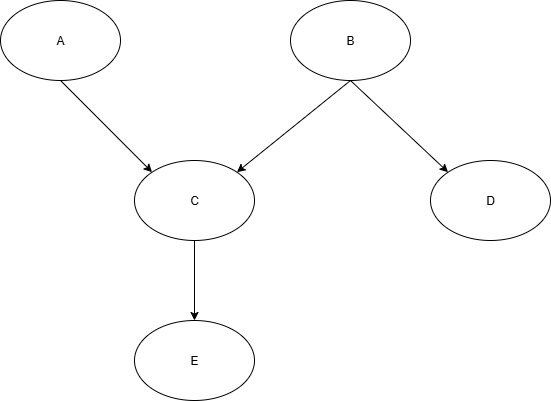
\includegraphics[width=\textwidth]{B_Network_Example.jpg}
 		\caption{Example of \acl{bn}}
 		\label{fig:bayesian_network}
 	\end{subfigure}
 	\hfill
 	\begin{subfigure}[b]{0.35\textwidth}
 		\centering
 		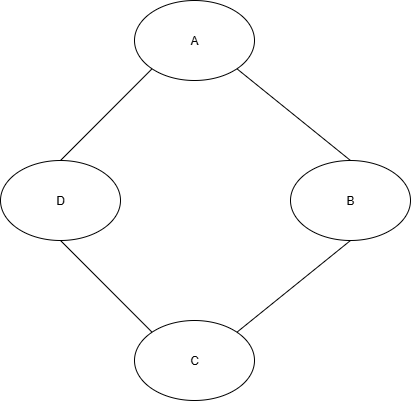
\includegraphics[width=\textwidth]{M_Network_Example.png}
 		\caption{Example of \acl{mn}}
 		\label{fig:markov_network}
 	\end{subfigure}
 	\caption{Examples of graphical models}
 	\label{fig:graph_networks}
 \end{figure}

In Figure~\ref{fig:bayesian_network}, the \acs{bn} is represented as a directed graph, where edges have arrows indicating conditional dependencies between random variables. A node with outgoing arrows is referred to as a parent, while nodes receiving those arrows are its children. For example, the arrow from node A to node C signifies that “C depends directly on A,” or equivalently, “A influences C.”

By contrast, the \acs{mn} in Figure~\ref{fig:markov_network} is undirected, with edges lacking any direction. This reflects symmetric dependencies: neither node is assumed to influence the other in a causal sense. In this case, the undirected edge between A and B indicates that “A and B are directly dependent,” without implying a specific direction of influence.

Finally, the last step is to define the factors required by the graph. For a \acs{bn}, each factor corresponds to a \acl{cpd} (\acs{cpd}), a conditional probability (\acs{pagb}) distribution for a variable given its parents. If a node has no parents, its factor is simply a marginal distribution \acs{pa}. For example, in the \acs{bn} from Figure~\ref{fig:bayesian_network}, the associated distributions are:

\begin{equation}P(A),  P(B),  P(C|A,B),  P(D|B),  P(E|C)\end{equation}

These are combined into one joint distribution (\acs{pjoint}) using the chain rule:

\begin{equation}P(A,B,C,D,E) = P(A).P(B).P(C|A,B).P(D|B).P(E|C)\end{equation}

This joint distribution can then be used like any other multivariate distribution.

While this approach is manageable for small networks, it becomes computationally expensive for larger ones. This is where inference comes in. The next section discusses how inference methods, particularly belief propagation, enable efficient probabilistic queries without explicitly computing full joint distributions.

\subsubsection{Inference}
Inference is the process of calculating probabilities of \acs{rv}s of interest given partial information. In practice, this means calculating the probability distribution of one \acs{rv} conditioned on observed evidence from other \acs{rv}s. This is very useful as in the real world not every \acs{rv} is observed, therefore the use of inference provides reason for unobserved \acs{rv}s.

All further explanations will be explained for \acs{bn} because they can be encoded into a \acs{mn}. This conversion from \acs{bn} to \acs{mn} involves removing the directional edges as well as making the inference more efficient. The conversion is achieved through moralization which is done in two steps:

\begin{enumerate}[label=\arabic*)]
	\item Connect all the parents of a common child - This means if two nodes have the same child an edge gets placed between them, also known as marrying the parents.
	\item All directional edges are dropped and replaced with undirected edges.
\end{enumerate}

 This method is shown as an example in Figure~\ref{fig:moral}, where it can be seen that the directed edges are converted to undirected edges and all parents who share children are joined.

\begin{figure}[htbp]
	\centering
	\begin{subfigure}[b]{0.45\textwidth}
		\centering
		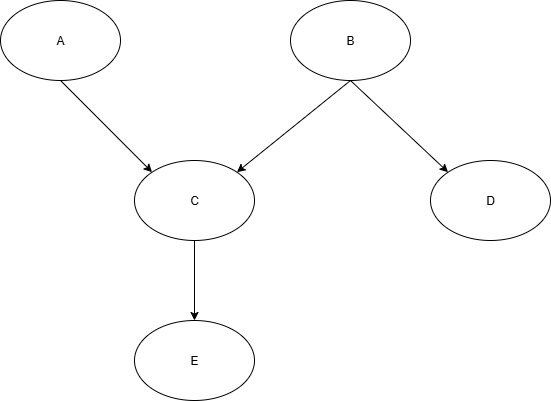
\includegraphics[width=\textwidth]{B_Network_Example.jpg}
		\caption{Example of \acl{bn}}
		\label{fig:bn}
	\end{subfigure}
	\hfill
	\begin{subfigure}[b]{0.45\textwidth}
		\centering
		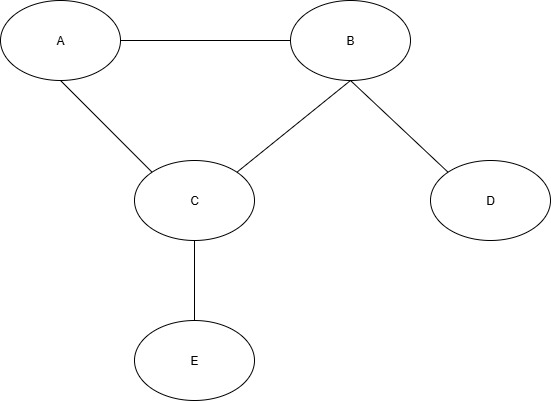
\includegraphics[width=\textwidth]{BN-MN.jpg}
		\caption{Example of \acl{mn} from a \acs{bn}}
		\label{fig:bn-mn}
	\end{subfigure}
	\caption{Conversion of \acl{bn} to \acl{mn}}
	\label{fig:moral}
\end{figure}

Now that all networks are \acs{mn}, the focus shifts to the two main methods of applying inference, \acl{bp} (\acs{bp}) and \acl{bu} (\acs{bu}). These two methods are very similar, with a few differences. 

\acs{bu} is typically applied to a single variable or a small set of variables, using Bayes' Theorem directly: 

\begin{equation}
\text{Posterior belief} = \frac{\text{Likelihood} \times \text{Prior belief}}{\text{Normalization factor}}
\end{equation}

The purpose of \acs{bu} is to refine the belief for a specific variable when new evidence arrives. This update is applied once per new observation, sequentially.

An example for this is if we looks at Figure~\ref{fig:bn-mn}. If evidence at D is observed, Bayesian Updating can be applied to compute the belief for B first, as B is directly connected to D, then the new belief of B can be used to update the beliefs of A and C, which can be extended as far as needed. 

In terms of mathematically explaining this, let evidence be observed at node $D$, denoted $D=d$. Using Bayesian Updating, we first update the belief for the neighboring node $B$:

\begin{equation}
P(B \mid D=d) = \frac{P(D=d \mid B) \, P(B)}{P(D=d)}
\end{equation}

where the normalization factor is

\begin{equation}
P(D=d) = \sum_B P(D=d \mid B) \, P(B).
\end{equation}


Next, we propagate the updated belief to the neighbors of $B$, namely $A$ and $C$:

\begin{equation}
P(A \mid D=d) = \sum_B P(A \mid B) \, P(B \mid D=d),
\end{equation}


\begin{equation}
P(C \mid D=d) = \sum_B P(C \mid B) \, P(B \mid D=d).
\end{equation}

Finally, the belief at $E$ can be updated via \acs{sum} over $C$:

\begin{equation}
P(E \mid D=d) = \sum_C P(E \mid C) \, P(C \mid D=d).
\end{equation}

This demonstrates sequential Bayesian Updating: starting from the observed evidence and propagating through the network to refine the beliefs of all connected nodes.

The other method is \acs{bp}, which is a message passing algorithm for inference in graphical models. This means that each node sends "messages" between each other about variables they have in common. The nodes then combine these messages into beliefs.

\subsubsection{Gaussian Factors}
For object tracking tasks such as in this project, Gaussian factors are especially useful as they can naturally represent noisy measurements of continuous variables, such as the ball's position across the video frames.
Gaussian factors often refer to factors or potential functions defined by a multivariate Gaussian distribution over a set of \acs{rv}. There are two main ways of describing Gaussian (Normal) distributions 

\begin{enumerate}
	\item Mean-Covariance form:\\
	\begin{equation}
	\mathcal{N}(x; \mu, \Sigma) = \frac{1}{(2\pi)^{n/2} |\Sigma|^{1/2}}\exp\left\{ -\frac{1}{2} (x - \mu)^T \Sigma^{-1} (x - \mu) \right\}
	\end{equation}
	where:
	\begin{itemize}
	\item $x$: Vector of \acs{rv}s
	\item $n$: Length of $x$  
	\item Mean ($\mu$): This is the "center" or average of the data.
	\item Covariance ($\Sigma$): This represents how much the values vary and how the different dimensions move together. A higher covariance on the main diagonal represents a lower confidence and large variance from the mean.
	\end{itemize}
	\item Canonical (Information) form:
	\begin{equation}
	C(x; K, h, g) = \exp\left\{ -\frac{1}{2} x^T K x + h^T x + g \right\}
	\end{equation}
	where:
	\begin{itemize}
	\item Information (Precision) Matrix $K$: Inverse of covariance, therefore a higher precision means lower uncertainty ($K = \Sigma^{-1}$)
	\item Information Vector $h$: Related to the mean ($h = K \mu$)
	\item Constant $g$: Adjusts the overall height but isn't always required.
	\end{itemize}
\end{enumerate}

The reason the canonical form is important for using Gaussian factors in a \acs{pgm} is that it allows for more efficient inference. Inference for Gaussian factors in \acs{pgm}s is performed via message passing on a cluster graph, following these steps:

\begin{enumerate}
	\item Create Cluster graph: Group all the factors together into "Clusters" connected by shared variables.
	\item Assign Factors to Clusters: Each cluster's "Potential" is a product of all the Factors assigned to it.
	\item Send messages between Clusters: Each message marginalizes out the cluster's private variables, passing only the shared variables into its neighbor.
	\item Compute Beliefs: Multiply incoming messages at each Cluster to get the final belief over its variables.
\end{enumerate}

\subsubsection{Hybrid Factors}
Hybrid networks are \acs{pgm}s that include both discrete and continuous \acs{rv}s within the same modeling framework. This needs to be discussed because pure discrete networks aren't able to handle continuous measurements, and pure continuous networks can't represent discrete measurements. This section discusses what happens when a network or model has both discrete and continuous \acs{rv}s.

Hybrid factors usually depicted mathematically as:

\begin{equation}\phi(x,y)\end{equation}

where:
\begin{itemize}
	\item $x$: Discrete \acs{rv}s
	\item $y$: Continuous \acs{rv}s
\end{itemize}

What this does is it handles the interaction between categorical decisions and real-valued outcomes. The joint distribution then factorizes as:

\begin{equation}p(x,y) = \prod_{i=1}^{n} \phi_i(X_i, Y_i)\end{equation}

where each factor $\phi_i$ can be either purely discrete, purely continuous or truly hybrid. This factorization is important as it enables inference and represents dependencies.

\paragraph{\acl{clg} (\acs{clg}) Networks}
\mbox{}\\
The most commonly used class of Hybrid Networks is a \acs{clg} network. A \acs{clg} network provides the structure to handle mixed discrete-continuous variables while keeping computational feasibility. A \acs{clg} network is generally preferred over general hybrid models as it is more tractable for inference, allowing for exact probabilistic computation rather than requiring approximation methods.

The \acs{clg} network is a hybrid network where:

\begin{itemize}
	\item Discrete variables can have any parents. (Discrete or Continuous)
	\item Continuous Variables with discrete parents follow a Gaussian distribution whose parameters depend on the parents.
	\item Continuous Variables with continuous parents must follow a linear Gaussian model.
\end{itemize}

\begin{figure}[H]
	\centering
	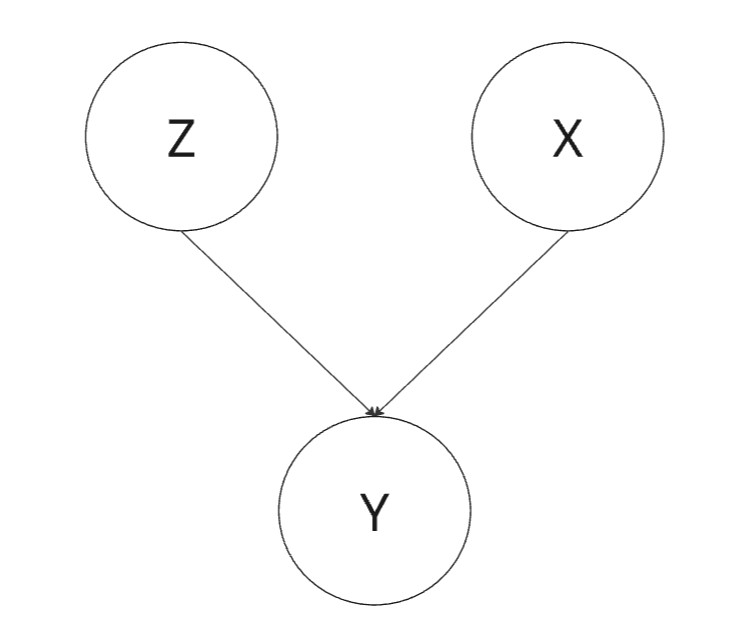
\includegraphics[width=0.4\textwidth]{hybridNet.jpg}
	\caption{Example of a \acl{clg} network showing discrete \acs{rv} $X$ and continuous \acs{rv}s $Y$ and $Z$}
	\label{fig:clg_network}
\end{figure}

A general setup of a \acs{clg} network is shown in Figure~\ref{fig:clg_network}, where $Y$ is a continuous \acs{rv} with discrete parent $X$ and continuous parent $Z$, the conditional distribution is given by:

\begin{equation}P(Y | Z, X=x) = N(Y; \mu_{x}(Z), \Sigma_{x})\end{equation}

where:

\begin{itemize}
	\item $\mu_{x}(Z) = a_{x} + b_{x}Z$ is a linear function of $Z$ with parameters depending on the discrete state $x$.
	\item $\Sigma_{x}$ is the covariance matrix also depending on $x$.
\end{itemize}

With all of this in mind, inference in \acs{clg} networks becomes more complex due to the mixture of discrete and continuous \acs{rv}s. This is where \acl{ep} (\acs{ep}) allows for easier inference.

\subsubsection{\acl{ep} (\acs{ep})}

\acs{ep} is a deterministic approximation technique for \acs{bn}s \parencite{minka2013ep}. \acs{ep} unifies two common approaches to inference techniques, the Kalman filter and Loopy \acs{bp}, which is an extension of previously mentioned \acs{bp} \parencite{minka2013ep}. The method of \acs{ep} is useful for Hybrid networks, as it approximates the belief states by retaining expectations such as means and variances \parencite{minka2013ep}.

\acs{ep} operates by approximating the posterior distribution through iterative moment matching between 'cavity' distributions (approximations excluding one factor's influence, denoted \(q_{-i}(x)\)) and 'tilted' distributions (cavity multiplied by the excluded factor, \(q_{-i}(x) \cdot f_i(x)\)). This process minimizes the Kullback-Leibler divergence \parencite{minka2001expectation,heskes2006approximate}.

\acs{ep} uses an iterative approach which in many cases is computationally infeasible. A special case of \acs{ep} is \acl{adf} (\acs{adf}) or commonly called Moment Matching. This method is done by initializing all the approximating factors except the first one to be uniform and then only allowing a single pass \parencite[510]{bishop2006prml}. This is necessary in the cases when data points arrive sequentially and the model must learn from each point and then discard the data before moving on to the next point \parencite[510]{bishop2006prml}.

Key steps for the \acs{adf} algorithm are as follows:

\begin{enumerate}
	\item \textbf{Initialization:} Start with simple approximations for all factors, assuming minimal prior knowledge.
	\item \textbf{Sequential processing:} Calculate the 'cavity' and 'tilted' distributions and then match moments of the 'tilted' distribution to the Gaussian distribution, updating the approximation immediately.
	\item \textbf{Single Pass:} Unlike the full \acs{ep}'s iterations, the \acs{adf} processes each data point once, discards it and then moves on to the next data point.
\end{enumerate}

\subsection{Gaps}
Despite advancements in commercial ball tracking systems and computer vision techniques, significant gaps remain in accessible, real-time solutions for sports analytics. High costs and infrastructure requirements of systems like Hawk-Eye limit their use beyond professional leagues, while open-source alternatives often lack the precision needed for reliable ball trajectory estimation. Additionally, integrating computer vision outputs with probabilistic graphical models for inference in hybrid networks presents challenges, particularly in handling occlusions, fast motion, and sequential data processing. Approximation methods like Expectation Propagation offer potential, but their computational demands and accuracy trade-offs in dynamic environments require further optimization for low-cost, real-time applications.

\newpage
\section{Model Design}
This section highlights the modular architecture, video footage, the role of \acp{pgm}, and the use of image processing algorithms. Figure~\ref{fig:model_overview} illustrates the overall pipeline of the system. The process begins with a sports video containing a ball. This video is passed through multiple image processing algorithms, each producing an independent estimate of the ball’s position. These outputs are then fused using a \acs{pgm}, which produces a final, unified estimate of the ball’s position.

\begin{figure}[H]
	\centering
	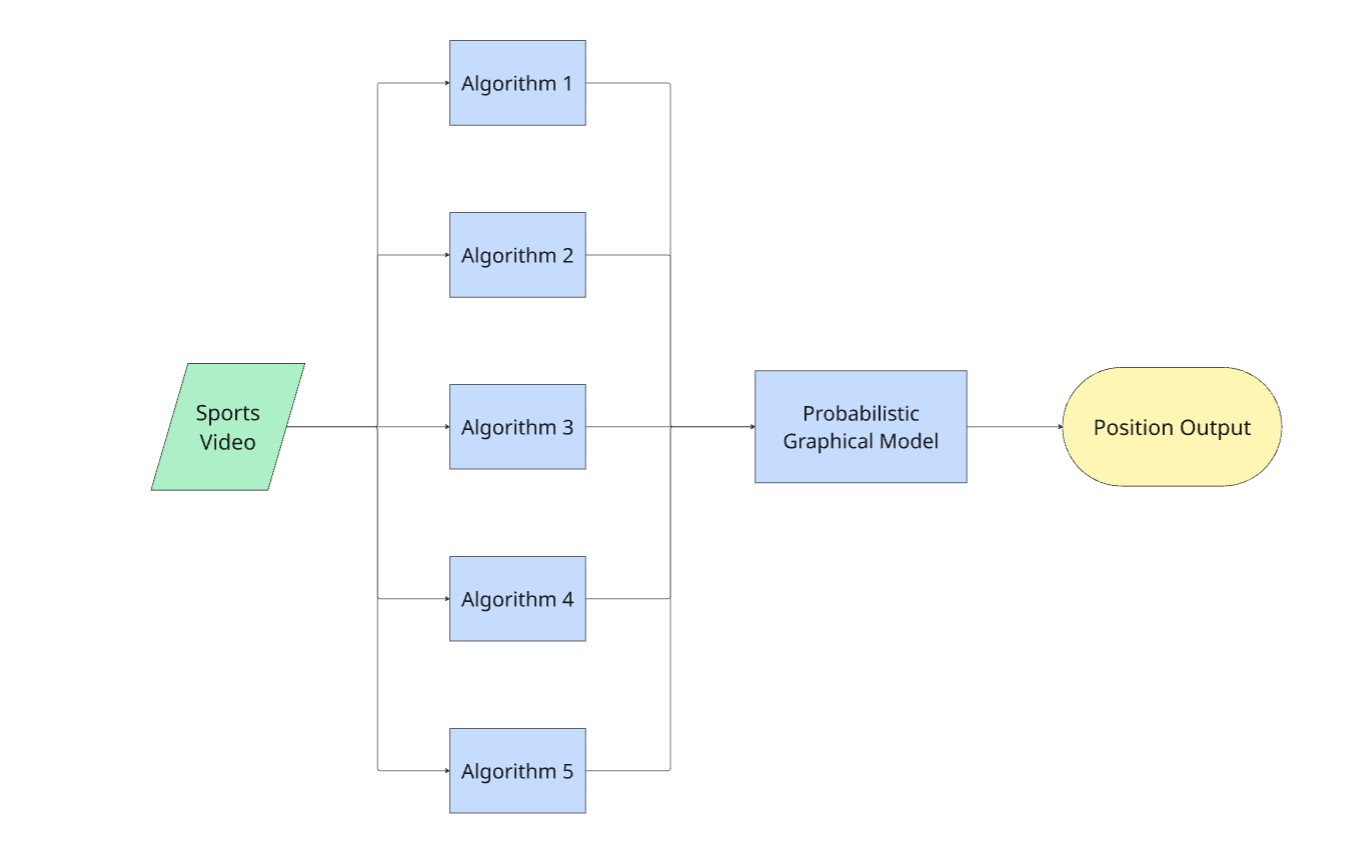
\includegraphics[width=1\textwidth]{ProjectOverview.jpg}
	\caption{Overview of the model design}
	\label{fig:model_overview}
\end{figure}

\subsection{Video Footage Description}

The sports video footage used in this project is sourced from a youtube video that displays a Court Level Tennis practice between Zverev and Djokovic \parencite{youtube_ZverevDjokovic}. The video is 43 minutes long and downloaded in MP4 at 1440p60 quality. The footage is captured at court level, with the camera positioned behind one of the players, where the ball is mostly visible and clearly identifiable. The video will be cut down into shorter video clips where the ball is in play, this is done to ensure manageable processing time, and will be using 30~\acl{fps} (\acs{fps}). The video will be pre-processed to ensure consistent lighting and colour balance, which helps improve the performance of the image processing algorithms.

\subsection{\acl{ipa}}
This subsection builds on the discussion of \acs{ipa} in the literature review (Section 2.3), where \acs{ipa}s are categorized into various levels. The purpose of \acs{ipa} in this project is to extract the raw data of the ball's position in each frame of the video and the reason for having multiple \acs{ipa} is to ensure that if one algorithm fails to detect the ball in a frame, the other algorithms and the \acs{pgm} can account for this failure and still provide reliable tracking of the ball. This subsection outlines the requirements needed of the \acs{ipa}, a discussion and design of the various candidate algorithms, and the differences in the algorithms. 

\subsubsection{Requirements}
To ensure that the \acs{ipa}s effectively support ball tracking, they must meet specific requirements. These requirements are derived from the project's needs for real-time performance and robustness to dynamic sports environments, building on the challenges discussed in the literature review. The key requirements for the \acs{ipa}s are outlined in Table~\ref{tab:ipa_requirements}. 

\begin{longtable}{@{} p{0.3\textwidth} p{0.65\textwidth} @{}}
    \caption{Requirements for Image Processing Algorithms}
    \label{tab:ipa_requirements} \\
        \toprule
        \textbf{Requirement} & \textbf{Description} \\
        \midrule
        \endfirsthead
        \toprule
        \textbf{Requirement} & \textbf{Description} \\
        \midrule
        \endhead
        \bottomrule
        \endfoot
        \bottomrule
        \endlastfoot
        Robustness to noise and distractions & The algorithm must reliably track the ball without getting "distracted" by background noise, such as players, lines on the fields or courts, or spectators. This ensures consistent detection in cluttered sports footage. \\
        
        Accuracy in ball center localization & The algorithm should precisely estimate the ball's center position, as well as minimizing errors that could affect trajectory prediction. \\
        
        Process video footage at 30~\acs{fps} & The algorithm must process frames at 30~\acs{fps} to support close to real-time tracking, maintaining efficiency for video analysis without significant time delays. \\
        
        Expand Scalability & The algorithm should handle varying video lengths, resolutions, and input formats with minimal performance degradation, allowing easy adaptation to diverse footage. \\
\end{longtable}

\subsubsection{Algorithm Design}
This subsection discusses the general design of the \acs{ipa}s (\acl{ipa}s), to ensure that the requirements in Section 3.2.1 are met. The design is presented as a Flow Diagram as per Figure~\ref{fig:ipaflow}, where the \acs{ipa} needs to be able to take in sports video footage, process each frame, and output an estimated position. The per-frame pixel coordinate $(x,y)$ is normalized by the frame width $W$ and height $H$ as follows:
\begin{equation}
x_{\mathrm{norm}} = \frac{x}{W}, \qquad y_{\mathrm{norm}} = \frac{y}{H}
\end{equation}
which maps positions into the unit square $[0,1]\times[0,1]$. The idea behind using $[-1,-1]$ is that the later \acs{pgm} will be able to identify easily that this input is not ideal and will ignore it since that specific algorithm didn't detect anything in that frame. These outputs then need to be outputted into a text file that can be used in the \acs{pgm}, where the naming of the text file will be \texttt{alg\_n.txt}, where $n \in \{1,...,N\}$ and $N$ is the number of algorithms used. Designing the general \acs{ipa} to work in this way satisfies several of the reqirements, being that it can process each frame at 30~\acs{fps}, it can easily be scaled to various video lengths, and it can be adapted to different video formats. The rest of the requirements will be met according to the specific Low-Level and Intermediate-Level operations used in each algorithm, the position of which can be seen in Figure~\ref{fig:ipaflow}.

\begin{figure}[H]
	\centering
	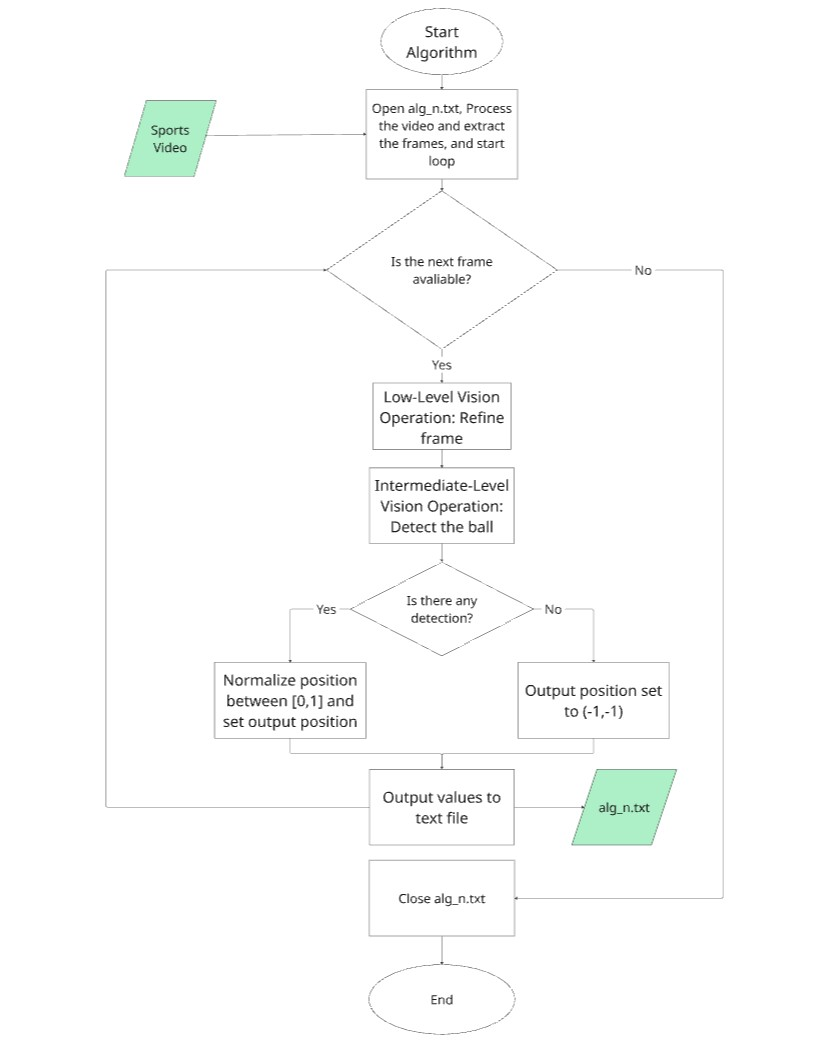
\includegraphics[width=0.75\textwidth]{ipa_flow.jpg}
	\caption{Flow diagram showing the flow of logic each of the \acs{ipa} will follow}
	\label{fig:ipaflow}
\end{figure}

\subsubsection{Candidate Algorithms}
This subsection discusses and guides the design of the various candidate algorithms that can be considered for this project. The functions and operations of these algorithms are based on the OpenCV library \parencite{opencv_library}, as discussed in Section 2.3.4. The aim of this subsection is to provide various combinations of operations that can be used to create different algorithms, which will then be tested and evaluated to determine the best performing algorithms for this project. The candidate algorithms are summarized in Table~\ref{tab:candidate_algorithms} and described further below the table.

\begin{longtable}{@{} p{0.15\textwidth} p{0.4\textwidth} p{0.4\textwidth} @{}}
\caption{Candidate Image Processing Algorithms}
\label{tab:candidate_algorithms} \\
    \toprule
    \textbf{Algorithm Name} & \textbf{Low-Level Vision Operation Used} & \textbf{Intermediate-Level Vision Operation Used} \\
    \midrule
    \endfirsthead
    \toprule
    \textbf{Algorithm Name} & \textbf{Low-Level Vision Operation Used} & \textbf{Intermediate-Level Vision Operation Used} \\
    \midrule
    \endhead
    \bottomrule
    \endfoot
    \bottomrule
    \endlastfoot
    \acs{hsv} Colour Thresholding & Median blur and morphological operations & Contour detection and shape analysis \\
    
    Motion Tracker & Frame differencing, thresholding, and morphological operations & Contour detection, ellipse fitting, and shape analysis \\
    
    Background Subtraction Tracker & Morphological operations & Background subtraction (MOG2), contour detection and shape analysis \\
    
    Canny Edge and Hough Circles & Canny edge detection & Hough circle transform \\
    
    Lucas-Kanade Optical Flow & N/A & Optical flow computation and feature tracking \\
    
    Template Matching & Template correlation & Localization \\
\end{longtable}

The descriptions for each algorithm are as follows:

    \textbf{\acs{hsv} Colour Thresholding:} This algorithm uses colour-based segmentation by converting the frame to a \acs{hsv} colour space. It applies median blur to reduce noise while preserving edges, followed by morphological operations like erosion and dilation to refine the binary mask. Contours are then detected, and shape analysis filters for circular shapes based on metrics like circularity and aspect ratio, making it effective for detecting the ball against varying backgrounds, however it may potentially be sensitive to lighting changes affecting colour perception.
    
    \textbf{Motion Tracker:} This algorithm focuses on motion detection. It computes frame differencing to highlight moving objects, applies thresholding to create a binary image, and uses morphological operations to clean up noise. It detects contours and fits ellipses to candidate shapes, then applies shape analysis to filter based on elongation and size, which is particularly useful for tracking fast-moving balls but may struggle with slow or stationary objects.
    
    \textbf{Background Subtraction Tracker:} This algorithm utilizes background modeling to separate foreground from background. It applies morphological operations to preprocess frames, uses MOG2 background subtraction to generate foreground masks, detects contours in the mask, and applies shape analysis to identify ball-like objects. It should be effective for static camera scenarios but may be affected by changing backgrounds or lighting variations.
    
    \textbf{Canny Edge and Hough Circles:} This algorithm detects edges using the Canny edge detector to identify object boundaries. It then applies the Hough circle transform to find circular shapes. It should be particularly suited for detecting the ball when it's well-defined and circular, offering geometric precision but potentially struggling with deformed or partially occluded balls.
    
    \textbf{Lucas-Kanade Optical Flow:} This algorithm implements sparse optical flow using the Lucas-Kanade method. It tracks feature points across frames to estimate motion trajectories. It should be ideal for following the ball's path over time, providing temporal continuity, but requires good feature initialization and may drift over long sequences.
    
    \textbf{Template Matching:} This algorithm uses correlation-based template matching to locate the ball by comparing a reference template against the frame. It should be straightforward and effective when the ball appearance is consistent, but can be computationally intensive and sensitive to scale, rotation, or appearance changes.

These algorithms all have been designed and tested to ensure the algorithms meet the requirements outlined in Section 3.2.1. All of these algorithms use low-level vision to remove noise and make the algorithms more robust and free from distractions. The intermediate-level vision operations are utilized to accurately determine the center of the ball's position. Therefore based on Figure~\ref{fig:ipaflow} and the descriptions above, these algorithms meet all of the requirements set.

\subsection{\acl{pgm}}
The purpose of incorporating \acp{pgm} in this project is to combine the outputs of multiple image processing algorithms in a principled and probabilistic manner. These algorithms, while effective individually, are not always reliable, they may occasionally fail to detect the ball or produce inaccurate estimations due to occlusion, motion blur, illumination variation or other visual disturbances. 

A \acs{pgm} allows for a robust fusion of these imperfect outputs by modeling both observed and latent variables, capturing the uncertainty inherent in each tracker’s prediction. This subsection presents the design and construction of the \acs{pgm} model used in the project, including its design requirements, structure, variable definitions, and how inference will be performed to estimate the ball's true position.

\subsubsection{Design Requirements}
In order to effectively design and implement the \acs{pgm} for this project, a clear set of requirements must be defined. These requirements provide a foundation for understanding how the model should be structured, what functionality it must support, and how the final output should behave. In particular, the requirements address aspects such as uncertainty handling, output quality, and model scalability. Table~\ref{tab:pgm_requirements} outlines the key requirements that the proposed \acs{pgm} must satisfy.

\begin{longtable}{p{0.3\textwidth} p{0.65\textwidth}}
\caption{Requirements for the Probabilistic Graphical Model} \label{tab:pgm_requirements} \\
\hline
\textbf{Requirement} & \textbf{Description} \\
\hline
\endfirsthead
\hline
\textbf{Requirement} & \textbf{Description} \\
\hline
\endhead
\hline
\endfoot
\hline
\endlastfoot
Handle uncertainty & The \acs{pgm} must account for noise or missing data in algorithm outputs by modeling them probabilistically. \\

Fuse multiple \acs{ipa}s & Must combine several algorithm outputs at each frame into a multivariate normal distribution. \\

Temporal consistency & The model should account for the smooth, continuous nature of the ball's motion by modeling how its position evolves over time, ensuring that current estimates depend on previous positions.\\

Scalable inference & The model must support efficient inference algorithms that remain computationally feasible as the video length increases or as additional tracking algorithms are integrated. \\

Modular design & The structure should allow easy integration or removal of trackers without changing the core model. \\

Factor structure & The relationships between variables must be clearly defined using Gaussian Distributions. \\
\end{longtable}

\subsubsection{Model Construction}
A \acs{bn} (\acl{bn}) was selected for this project as its strengths lie in its ability to explicitly model the dependencies between variables through the use of directed edges. This is \acs{bn}s strength when compared with \acs{mn} for this project, while both can represent complex dependencies and perform inference under uncertainty \parencite{koller2009pgm}, the causal reasoning of the \acs{bn} works well for this project as the image processing algorithms depend on the actual position of the ball.

\textbf{Random Variables}

There are 3 \acs{rv}s per time step, these are presented in Table~\ref{tab:rvs}. 

\begin{longtable}{p{0.15\textwidth} p{0.25\textwidth} p{0.3\textwidth} p{0.2\textwidth}}
\caption{Random Variables for the Probabilistic Graphical Model} \label{tab:rvs} \\
\hline
\textbf{RV} & \textbf{Symbol} & \textbf{Description} & \textbf{Domain} \\
\hline
\endfirsthead
\hline
\textbf{RV} & \textbf{Symbol} & \textbf{Description} & \textbf{Domain} \\
\hline
\endhead
\hline
\endfoot
\hline
\endlastfoot
		Ball position & $Pos_{x,y}$ & Actual position of the ball on the screen in normalized coordinates (x and y values) & $[0, 1] \times [0, 1]$ \\
		Algorithm outputs & $Alg_n$ (for $n=1,...,N$) & Output from the $n$-th image processing algorithm & $[0, 1] \times [0, 1]$ \\
		Outlier Indicator & $a_n$ (for $n=1,...,N$) & Discrete \acs{rv} indicating if $Alg_n$ is an outlier & $\{0 = \text{outlier}; 1 = \text{inlier}\}$ \\
\end{longtable}

Since each image processing algorithm typically outputs a single $(x, y)$ position estimate, this alone does not provide a continuous distribution over all possible ball locations. To meet the requirement of a multivariate normal distribution in the model, a Gaussian factor is applied to each algorithm’s output. This is done by taking the algorithm's output as the mean $\mu_n$ of a multivariate Gaussian distribution and associating it with a covariance matrix $\Sigma_n$ that captures the algorithm's expected positional uncertainty. The specific values for these covariance matrices, along with temporal motion parameters and outlier probability priors, will be determined through systematic evaluation in Chapter 5.

This transforms the single point estimate into a probabilistic relationship, centered around the algorithm's prediction with an associated covariance that represents its uncertainty. The resulting domain for each algorithm’s output becomes $[0,1]\times[0,1]$, with a continuous distribution that reflects the inherent error or noise in the algorithm's estimate.

Sometimes the algorithms may produce irregular or wrong outputs, for example if the ball is occluded or there are distractions within the frame then one of the \acs{ipa} may output a position that is far from the actual ball position. To account for this the \acs{pgm} includes a discrete \acs{rv} called $a_n$ for each individual \acs{ipa}. This \acs{rv} indicates if the output is an outlier or inlier, this therefore produces a Hybrid network as there are now both discrete and continuous \acs{rv}s.

\textbf{Relationships}

Now that the \acs{rv}s have been defined, the next step is to define the relationships between them. It is evident that the output of each algorithm directly depends on the actual position of the ball as well as whether the output is an outlier. Therefore, there is a causal relationship between $Pos_{x,y}$ and $Alg_n$ and between $a_n$ and $Alg_n$, as illustrated in Figure~\ref{fig:smallBN}. This implies that the algorithm outputs are conditionally dependent on both the true ball position and the Outlier Indicator.

\begin{figure}[H]
	\centering
	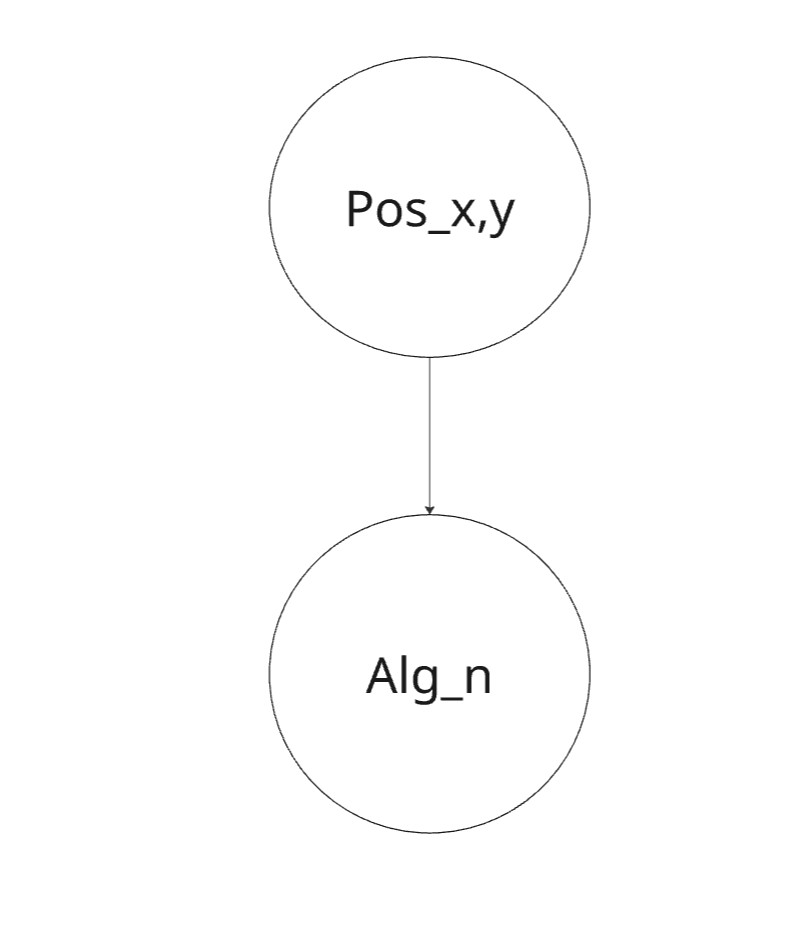
\includegraphics[width=0.35\textwidth]{smallBN.jpg}
	\caption{Relationship between $Pos_{x,y}$, $Alg_n$ and $a_n$ for single algorithm and time step}
	\label{fig:smallBN}
\end{figure}

With this in mind, the full model can be defined as shown in Figure~\ref{fig:fullBN}. This represents the final \acs{bn} design used in this project for a single time step. (While the example illustrates five algorithms, the final number is still to be confirmed.)

\begin{figure}[H]
	\centering
	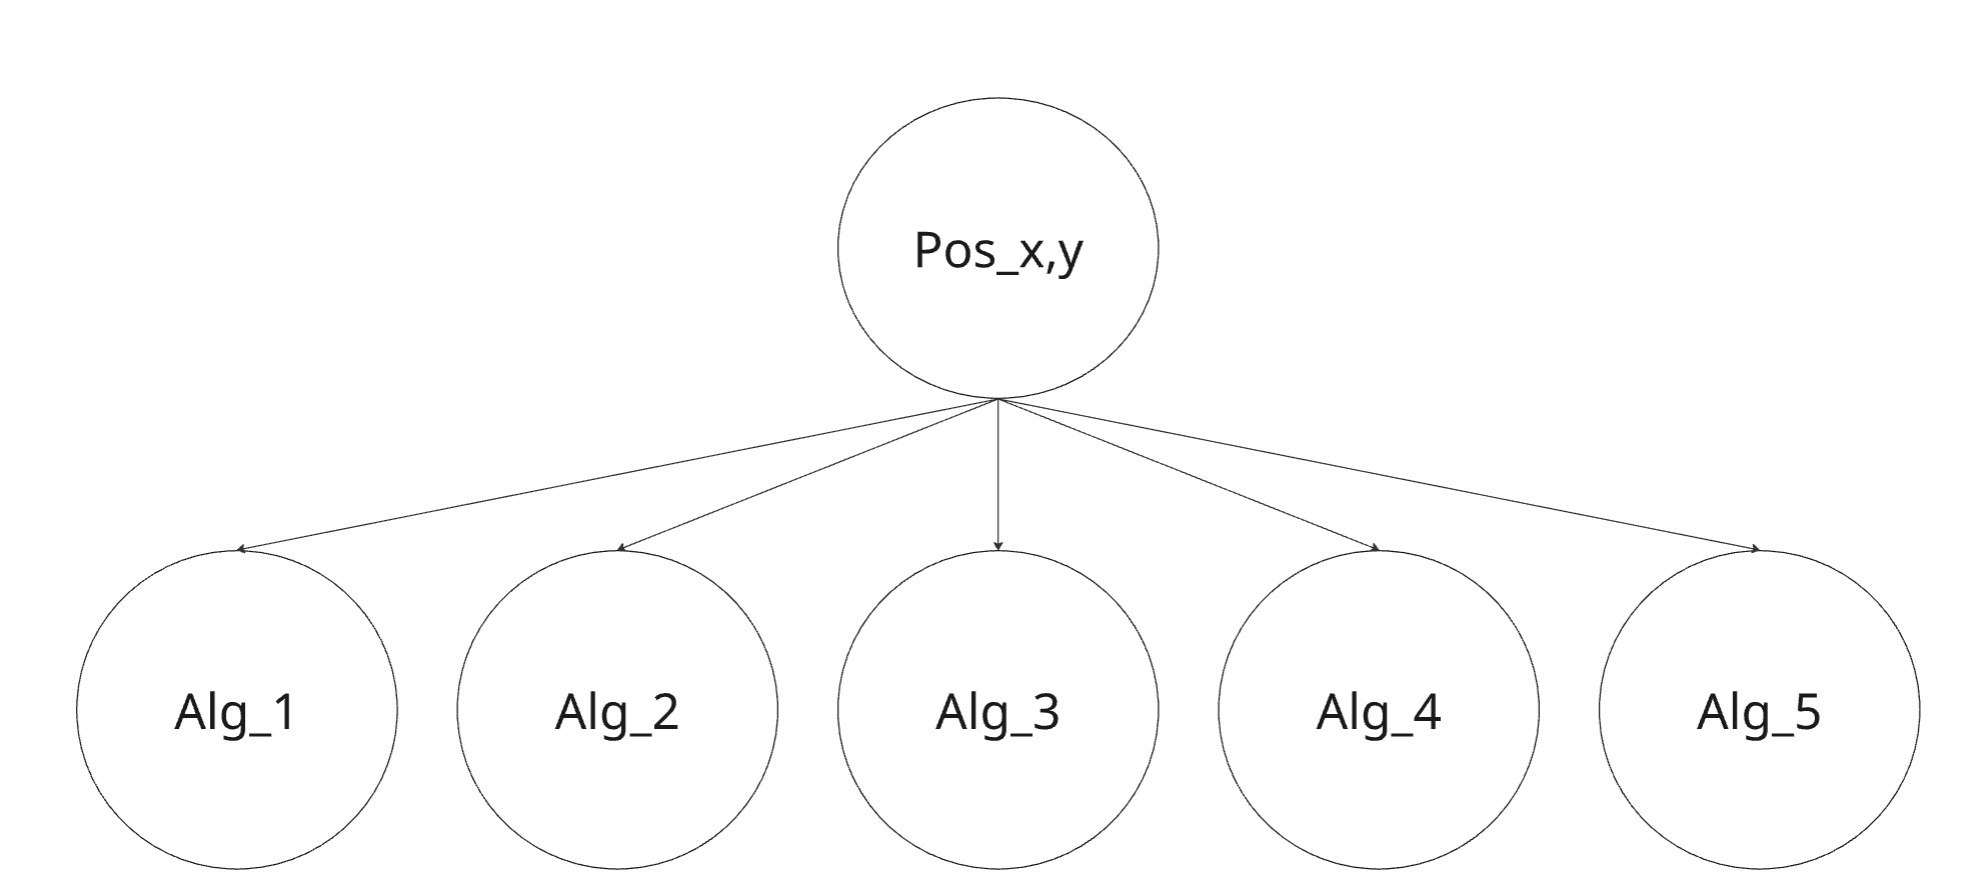
\includegraphics[width=0.5\textwidth]{fullBN.jpg}
	\caption{\acl{bn} showing the relationships between $Pos_{x,y}$ and the various algorithms used}
	\label{fig:fullBN}
\end{figure}

\textbf{Time-step connections}

At this point in order for the ball to be tracked smoothly and efficiently the other frames need to be taken into account. This will be done with $Pos_{x,y}$ having a direct influence on the same \acs{rv} in the next time step. From here the use of $Pos_{x,y}1$, $Pos_{x,y}2$, ..., $Pos_{x,y}n$ will be used per time step. Figure~\ref{fig:fulltimeBN} shows the relationships between each time step. As can be seen, $Pos_{x,y}1$ has direct influence on $Pos_{x,y}2$, this means that the position of the ball in the next frame is dependent on the position of the ball in the current frame. This is important as it ensures that the ball's motion is modeled smoothly over time, reflecting its continuous trajectory across frames.
 
 \begin{figure}[H]
 	\centering
 	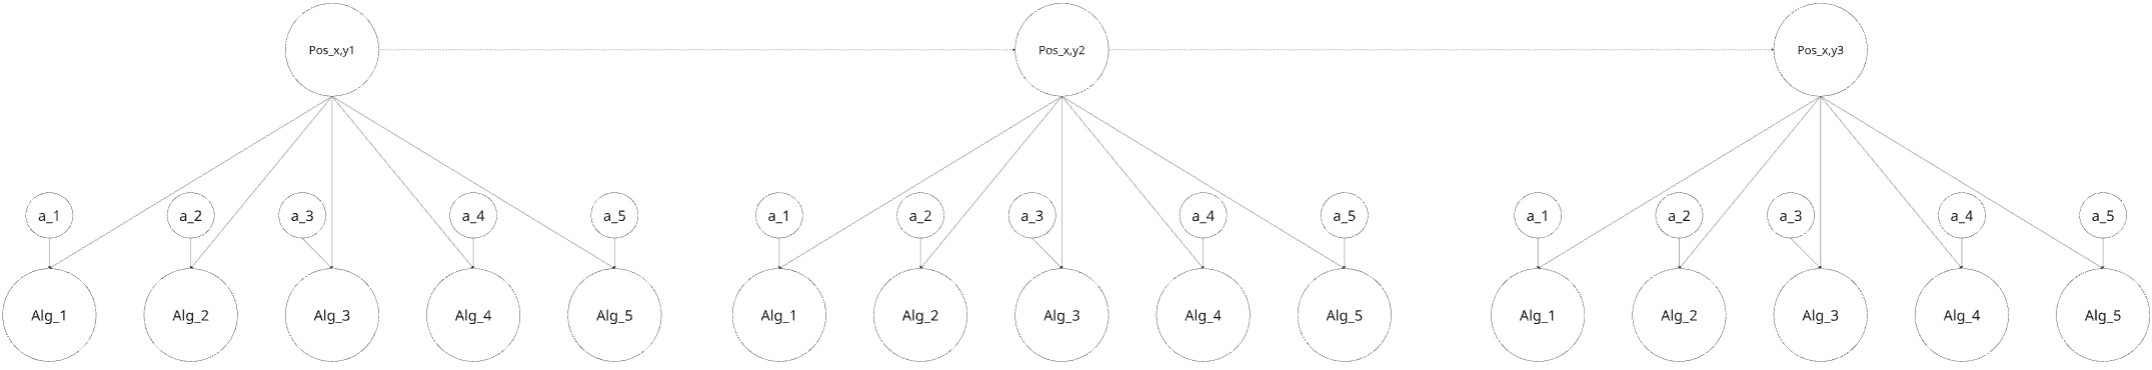
\includegraphics[width=1\textwidth]{BNwtime.jpg}
 	\caption{\acl{bn} showing the relationships between $Pos_{x,y}$, the various \acs{ipa} used and the discrete Outlier Indicators at the different time steps}
 	\label{fig:fulltimeBN}
 \end{figure}

 
\textbf{Factor Definitions}

The probabilistic relationships in the \acs{bn} are formalized through the following factor definitions:

\begin{itemize}
	\item Temporal dynamics factor modeling the ball's motion between consecutive frames
	\begin{equation}P(Pos_{x,y}^t | Pos_{x,y}^{t-1})\end{equation}
	\item Observation model factor relating algorithm outputs to true position and outlier status
	\begin{equation}P(Alg_n | Pos_{x,y}, a_n)\end{equation}
	\item Outlier prior factor representing the probability that algorithm $n$ produces an outlier
	\begin{equation}P(a_n)\end{equation} 
\end{itemize}

These factors define the conditional dependencies within the hybrid network.

\textbf{Mathematical Specification}

These factor definitions now need to be formalized as Gaussian distributions. The mathematical specifications for the factors are as follows:

\begin{itemize}
	\item Temporal dynamics factor:
	\begin{equation} P(Pos_{x,y}^t | Pos_{x,y}^{t-1}) = \mathcal{N}(Pos_{x,y}^t; Pos_{x,y}^{t-1}, \Sigma_{motion}) \end{equation}
	\item Observation model:
	\begin{equation}
	P(Alg_n | Pos_{x,y}, a_n) = \begin{cases}
	\mathcal{N}(Alg_n; Pos_{x,y}, \Sigma_n) & \text{if } a_n = 1 \text{ [inlier]} \\
	\mathcal{N}(Alg_n; c, \Sigma_o) & \text{if } a_n = 0 \text{ [outlier]}
	\end{cases}
	\end{equation}
	where:
	\begin{itemize}
		\item $c$: A constant mean.
		\item $\Sigma_o$: A large covariance matrix representing high uncertainty for outliers.
	\end{itemize}
\end{itemize}

 \subsubsection{\acs{pgm} Design}
This subsection discusses the design flow of the \acs{pgm}, as shown in Figure~\ref{fig:pgmflow}. The model should begin by reading the \acs{ipa} outputs from their text files. For each time step (Frame), the model needs to set all of the initial means and covariance matrices. From there each the model should loop through each algorithm and perform \acs{ep} to update the belief about the ball's position based on each algorithm's output and its outlier status. \acs{ep} needs to be done here as this model is a Hybrid network and regular \acs{bp} will not work for this model. The beliefs or messages are then fused from the last algorithm via Moment Matching as the inference method used is \acs{ep} therefore there will be multiple difference guassians fusing messages together. Finally the outputs need to be converted to Mean-Covariance form and outputted to a text file that can be used for evaluation and to be overlayed with the original video footage to show the tracking.
 
\begin{figure}[H]
	\centering
	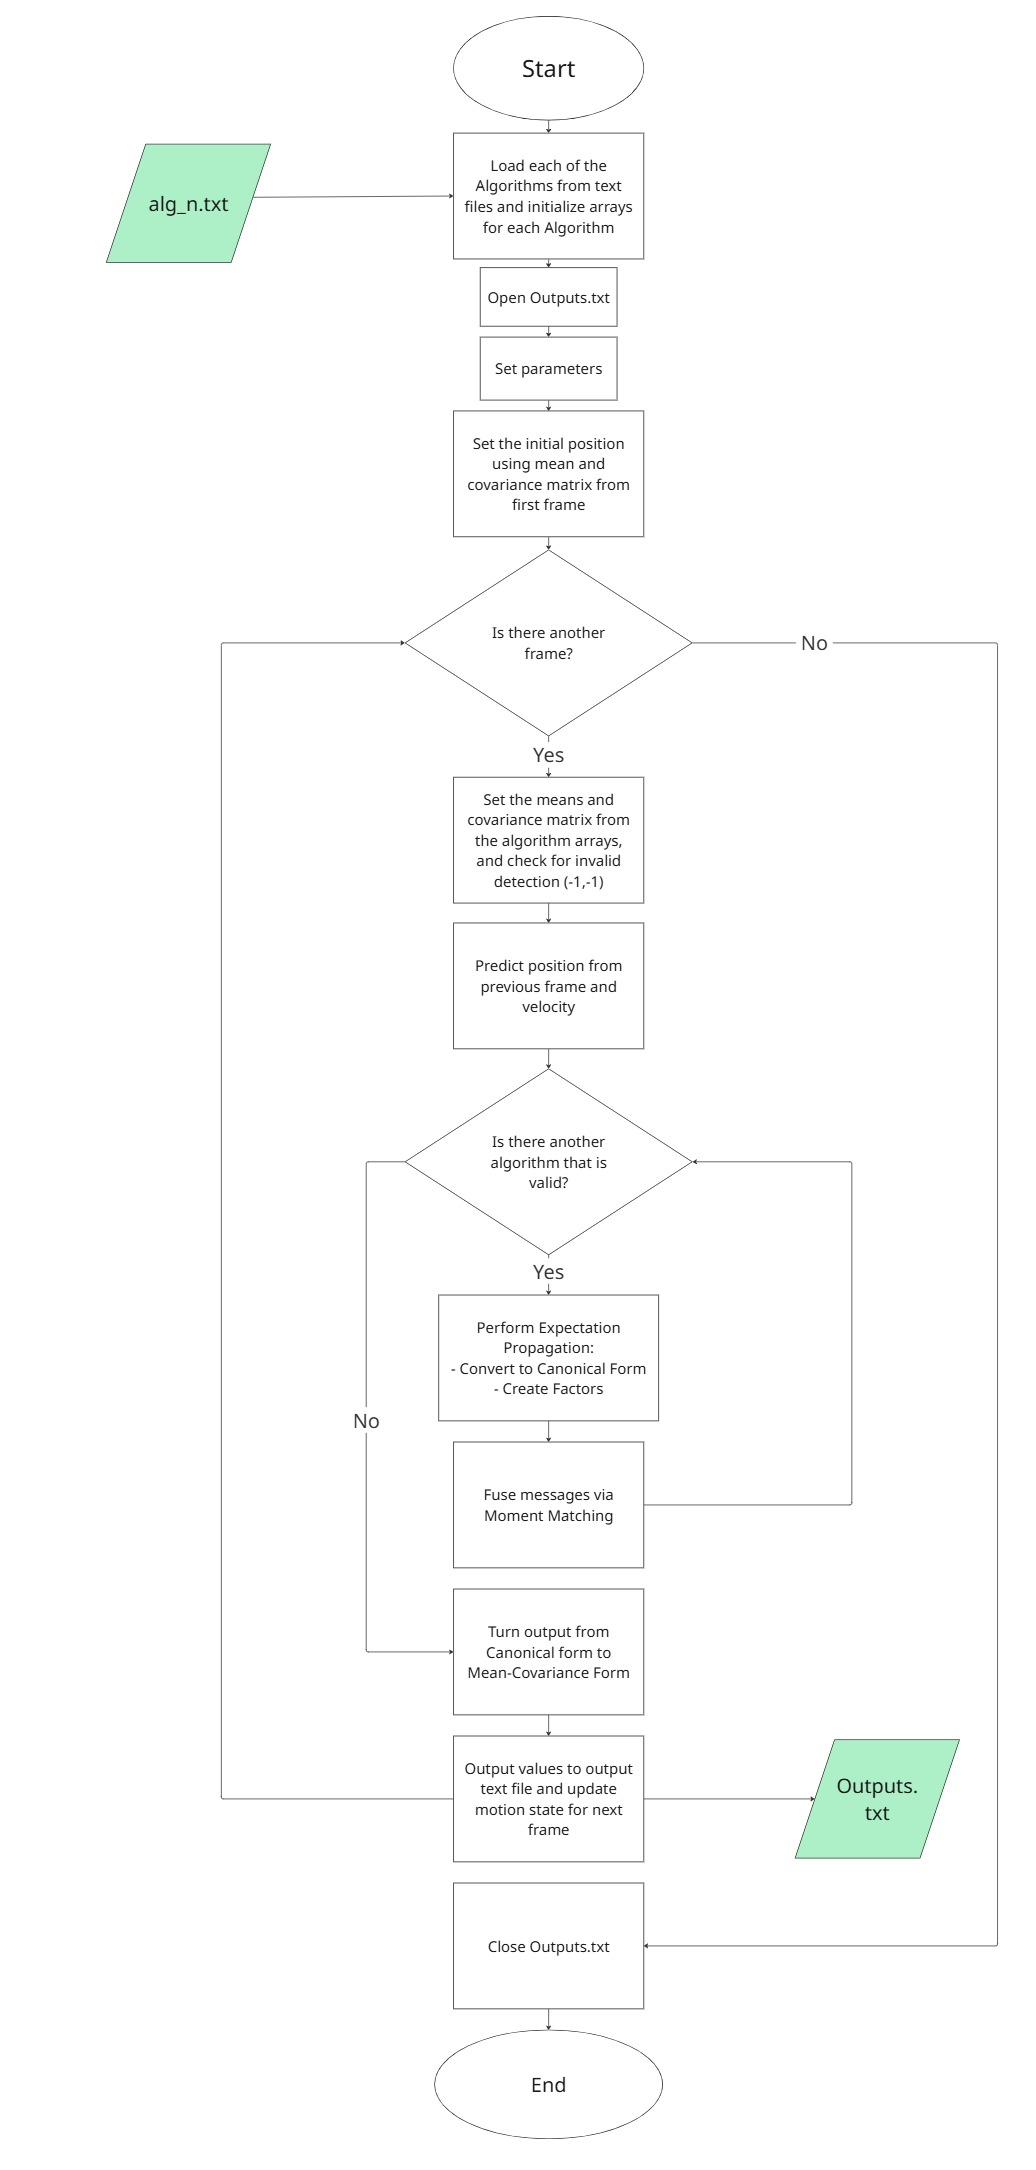
\includegraphics[width=0.75\textwidth]{pgmflowdesign.jpg}
	\caption{Flow diagram showing the flow of logic the \acs{pgm} will follow}
	\label{fig:pgmflow}
\end{figure}

 \newpage
\section{Implementation}
This chapter discusses the implementation of the ball tracking system, focusing on \acs{ipa} (\acl{ipa}), \acs{pgm} (\acl{pgm}), and the way the two will communicate together and how data will flow through them. The chapter opens on the discussion of \acs{ipa} implementation, followed by the implementation and foundations for how the \acs{pgm} will be implemented. Finally, the chapter concludes with a discussion on how the system is integrated and how the data will flow throughout the system.

\subsection{\acs{ipa} Implementation}
This subsection will detail the practical implementation of the \acs{ipa} discussed and designed in Section 3.2. It will detail the \acs{ipa}s implementation and Code architecture, parameter selection, output specification for each candidate algorithm and then final selection of algorithms. The implementation will ensure processing at 30~\acs{fps} while maintaining robustness to noise, distractions, or other factors which may affect tracking.

Based on the candidate algorithms discussed in Section 3.2.3, these \acs{ipa}s will be implemented and tested. The final selection will be based on their strengths when compared with the other \acs{ipa}, ensuring the selected algorithms complement each other in terms of ensuring the ball is tracked every frame by at least one algorithm and aren't too computationally heavy.

\subsubsection{Implementation and Code Architecture}
This subsection details the implementation of the \acs{ipa}s described in Section 3.2.3. All implementations are developed in Python utilizing the OpenCV library \parencite{opencv_library} for computer vision operations.

Each \acs{ipa} employs \texttt{cv2.VideoCapture} to process video footage frame-by-frame. Frames are analyzed according to the algorithm's design, with shared parameters including HSV bounds of $[27, 15, 150]$ to $[80, 255, 255]$, which are derived through iterative sampling of the ball's color across varying lighting conditions and the area constraints of $[20, 150]$ pixels, established via pixel counting at different distances to accommodate ball size variations. Pseudocode for these algorithms is provided in Appendix B.

If no ball is found in the algorithm, the output is set to $(-1,-1)$. Once the algorithm is done processing the outputs are written to a text file with naming convention of \texttt{alg\_n.txt}, where $n$ is the algorithm number. These algorithms will all be tested and evaluated in Chapter 5 to determine the best performing algorithms for this project. The final selection of algorithms will be confirmed in the Chapter 5.


\paragraph{\acs{hsv} Colour Thresholding}
\mbox{}\\
The HSV Colour Thresholding algorithm forms the foundation of the system's low-level vision pipeline, leveraging colour segmentation for robust ball detection under varying illumination. Implemented in Python with OpenCV, it processes each frame sequentially, starting with noise reduction and progressing to shape-based filtering. The core architecture emphasizes modularity: colour conversion isolates the ball, morphological operations refine the mask, and contour analysis selects the most probable candidate based on geometric properties.

The processing pipeline begins with median blurring to preserve edges while suppressing noise, using \texttt{cv2.medianBlur}.

Colour space conversion to HSV enables threshold-based segmentation, invariant to brightness variations: \texttt{cv2.cvtColor} and \texttt{cv2.inRange}.

Morphological dilation and erosion refine the binary mask, filling gaps and removing distortions, using a 3x3 rectangular kernel: \texttt{cv2.dilate} and \texttt{cv2.erode}.

At the intermediate level, contour detection identifies potential ball regions, with selection criteria prioritizing circularity and solidity (area ratio to convex hull) to distinguish the ball from elongated or irregular shapes. A weighted scoring system ranks contours, selecting the top candidate and normalizing its centroid to $[0,1]$ for PGM integration.

\paragraph{Motion Tracker}
\mbox{}\\
The Motion Tracker algorithm detects and tracks the ball by combining motion detection with shape analysis, making it effective for fast-moving objects in dynamic scenes. Implemented in Python with OpenCV, it processes frames by first isolating motion through differencing, then refining with color cues and contour filtering.

The algorithm starts by converting frames to grayscale and HSV for dual processing: \texttt{cv2.cvtColor}.

Frame differencing highlights moving regions using absolute difference and thresholding: \texttt{cv2.absdiff} and \texttt{cv2.threshold}.

Finally the algorithm combines the masks via bitwise operations and isolates the ball:\\ \texttt{cv2.bitwise\_and}.

Contour detection and shape analysis apply the same criteria as \acs{hsv} Colour Thresholding (area, circularity, aspect ratio, solidity), prioritizing elongated shapes from motion streaks. The top-ranked contour's centroid is normalized to $[0,1]$ for PGM integration. 

\paragraph{Background Subtraction Tracker}
\mbox{}\\
The Background Subtraction Tracker leverages background modeling to identify foreground motion, ideal for static camera setups. Using OpenCV's MOG2 algorithm, it separates moving objects from the background, combining this with color filtering for robust ball isolation.

Initialization sets up the subtractor with tuned parameters:\\ \texttt{cv2.createBackgroundSubtractorMOG2}.

Each frame is processed with HSV color masking and background application: \texttt{cv2.cvtColor}, \texttt{cv2.inRange}, and the subtractor's \texttt{apply} method.

Masks are combined and refined with morphological opening: \texttt{cv2.bitwise\_and} and \texttt{cv2.morphologyEx}.

Contour detection uses the same selection criteria as HSV Colour Thresholding (area, circularity, aspect ratio, solidity), normalizing the best match to $[0,1]$. 

\paragraph{Canny Edge and Hough Circles}
\mbox{}\\

The Canny Edge and Hough Circles algorithm detects the ball through geometric shape recognition, focusing on circular edges for precise localization. Implemented in OpenCV, it preprocesses frames with color masking and blurring before applying edge detection and circle fitting.

Frame preprocessing involves HSV color masking and morphological cleanup: \texttt{cv2.cvtColor}, \texttt{cv2.inRange}, and \texttt{cv2.morphologyEx}.

Grayscale conversion and Gaussian blurring prepare for edge detection: \texttt{cv2.GaussianBlur}, and \texttt{cv2.bitwise\_and}.

Canny edge detection identifies boundaries, followed by dilation for completeness: \texttt{cv2.Canny} and \texttt{cv2.dilate}.

The Hough Circle Transform detects circles with tuned parameters: \texttt{cv2.HoughCircles}.

The best circle's center is selected and normalized to $[0,1]$ if detected.

\paragraph{Lucas-Kanade Optical Flow}
\mbox{}\\

The Lucas-Kanade Optical Flow algorithm tracks the ball by estimating feature point motion across frames, providing temporal continuity for dynamic trajectories. Using OpenCV's sparse optical flow, it initializes and updates points within color-masked regions.

Parameters are set for robust tracking using dictionaries for optical flow and feature detection.

Frames are preprocessed with color masking and morphology: \texttt{cv2.cvtColor}, \texttt{cv2.inRange}, and \texttt{cv2.morphologyEx}.

Feature detection and optical flow computation track points: \texttt{cv2.goodFeaturesToTrack} and \texttt{cv2.calcOpticalFlowPyrLK}.

Valid points within the mask are filtered, and their centroid is calculated and normalized to $[0,1]$ if sufficient points are tracked.

\paragraph{Template Matching}
\mbox{}\\

The Template Matching algorithm locates the ball by correlating a reference template with each frame, offering straightforward detection when appearance is consistent. Using OpenCV's normalized cross-correlation, it preprocesses frames and applies a similarity threshold.

The template is loaded and prepared: \texttt{cv2.imread}.

Frames are masked and matched: \texttt{cv2.cvtColor}, \texttt{cv2.inRange}, \texttt{cv2.bitwise\_and}, and \texttt{cv2.matchTemplate}.

The best match is located and thresholded: \texttt{cv2.minMaxLoc}.

The center is normalized to $[0,1]$ if above threshold.

\subsection{\acs{pgm} Implementation}
This section describes the practical realization of the \acs{pgm} framework designed in Section 3.3. It addresses three principal challenges: representing Gaussian factors in a stable form suitable for message passing, performing \acs{ep} on the hybrid \acs{bn}, and handling the mixture model for probabilistic outlier rejection. The following subsections discuss the key technical decisions, algorithmic adaptations, and numerical considerations that enabled a robust and efficient implementation.

\subsubsection{Software Framework and Architecture}
The tracker was implemented in C++ to leverage computational efficiency and precision required for ball tracking processing. The implementation builds upon the EMDW framework developed at Stellenbosch University \parencite{emdw_repo}, which provides foundational infrastructure for probabilistic graphical models. The Prlite library within EMDW supplies matrix and vector data structures \\(\texttt{RowMatrix}, \texttt{ColVector}), and the Eigen library provides linear algebra operations for matrix inversion and determinant computation.

This dual library approach was adopted because the Prlite matrices integrate well with EMDW's probabilistic modeling framework, while the Eigen library offers numerical algorithms for critical operations. Conversion functions bridge the two representations, transforming matrices between libraries only when necessary to minimize computational overhead.

\subsubsection{Canonical Form Representation}
The implementation employs Canonical (Information) form of Gaussian distributions rather than Mean-Covariance form. A Gaussian distribution in Canonical form is represented by its precision matrix and information vector. As shown in Equation 20 and 21 these are calculated using the mean $\mu$ and covariance $\Sigma$ from the Mean-Covariance form:

\begin{equation}
\Lambda = \Sigma^{-1}
\end{equation}

\begin{equation}
h = \Lambda\mu
\end{equation}

This representation offers significant advantages for \acs{ep} message passing. Product operations, which occur frequently during belief updates, reduce to simple addition in canonical form as shown in Equation 22.
\begin{equation}
\mathcal{N}(x; \mu_1, \Sigma_1) \times \mathcal{N}(x; \mu_2, \Sigma_2) \propto \mathcal{N}(x; \Lambda_1 + \Lambda_2, h_1 + h_2)
\end{equation}

Similarly the division operations, required for cavity computation, become subtractions. This eliminates the need for repeated matrix inversions that would dominate the computational cost. The posterior distribution and all factor messages are maintained in canonical form throughout inference, with conversion to Mean-Covariance form performed only at the final output stage.

\subsubsection{Expectation Propagation Inference}
Standard \acs{bp} algorithms are unsuitable for a hybrid network such as this one, being unable to effectively handle the mixture of discrete outlier indicators $a_n$ coupled with continuous position variables. \acs{ep} provides an approximate inference framework that marginalizes over discrete variables while maintaining tractable Gaussian beliefs over continuous variables.

The idea behind the next 2 subsections is that the \acs{ep} tracker refines position estimates by: removing each algorithm's contribution (cavity), evaluating mixture components via Bayesian weighting, collapsing to a single Gaussian through moment matching, and updating messages in canonical form. This process automatically reduces the number of outliers through Mahalanobis distance based weighting while the canonical form ensures stability through efficient matrix operations. The result is a robust fusion method that adapts to varying measurement quality without manual tuning.

\textbf{Cavity Distribution Computation}

At each iteration for algorithm $n$, \acs{ep} constructs a cavity distribution $q_{-n}(x)$ by removing the current factor's contribution from the posterior. In canonical form, this is computed as:

\begin{equation}
\Lambda_{-n} = \Lambda_q - \Lambda_n
\end{equation}
\begin{equation}
h_{-n} = h_q - h_n
\end{equation}

where $\Lambda_q$ and $h_q$ represent the current posterior, and $\Lambda_n$ and $h_n$ are the message parameters from algorithm $n$. The cavity distribution serves as the prior for evaluating the mixture model in the next step.

\textbf{Message Update}

After computing the tilted distribution (described later in this subsection under the Mixture-Based Outlier Model), the new message is obtained by division. Since the distributions are in canonical form, this division operation reduces to subtraction:
\begin{equation}
\Lambda_n^{\text{new}} = \Lambda_{\text{tilt}} - \Lambda_{-n} 
\end{equation}
\begin{equation}
h_n^{\text{new}} = h_{\text{tilt}} - h_{-n}
\end{equation}

This update ensures the algorithm incorporates new information from each algorithm. The posterior is then updated by incorporating these new message:
\begin{equation}
\Lambda_q = \Lambda_{-n} + \Lambda_n 
\end{equation}
\begin{equation}
h_q = h_{-n} + h_n
\end{equation}

This direct update approach ensures that each algorithm's contribution is fully reflected in the posterior after a single pass through all measurements, making the inference efficient for sequential processing.

\textbf{Mixture-Based Outlier Model}

Each algorithm's measurement likelihood is modeled as a two-component Gaussian mixture that marginalizes over the discrete outlier indicator $a_n$ and weights $w_{\pi,a}^{(n)}$ representing the prior probability of each component. The mixture model is defined as follows:
\begin{equation}
p(Alg_n | Pos_{x,y}) = w_{\pi,\text{outlier}}^{(n)} \cdot \mathcal{N}(Alg_n; Pos_{x,y}, \Sigma_{\text{outlier}}) + w_{\pi,\text{inlier}}^{(n)} \cdot \mathcal{N}(Alg_n; Pos_{x,y}, \Sigma_n)
\end{equation}
where:
\begin{itemize}
    \item The outlier component (first term) has a large covariance $\Sigma_{\text{outlier}} = \sigma_0^2 I$ with $\sigma_0^2 = 1.0$, representing high uncertainty when the algorithm produces an invalid measurement. 1.0 is selected as it covers the entire normalized image space, effectively treating outliers as uniformly distributed.
    \item The inlier component (second term) has algorithm-specific covariance $\Sigma_n$, representing the regular covariance matrix of algorithm $n$ under normal conditions.
\end{itemize}

\textbf{Bayesian Component Weighting}

An updated weight for each component is computed using Bayes' rule, incorporating both the prior mixture weights $w_{\pi,a}^{(n)}$ and the likelihood that this position is an outlier. This is done to determine how much each component should influence the final estimate.\\

The weights are computed as follows as per \parencite[pg.~438-439]{bishop2006prml}:

\begin{equation}
w_a \propto w_{\pi,a}^{(n)} \cdot \mathcal{N}(\text{Alg}_n; \mu_{-n}, \Sigma_{-n} + \Sigma_a^{(n)})
\end{equation}

To ensure numerical stability, weights are computed in log-space also from \parencite[pg.~438-439]{bishop2006prml}:

\begin{equation}
\log w_a = \log w_{\pi,a}^{(n)} - \frac{1}{2}\log|\Sigma_{-n} + \Sigma_a^{(n)}| - \frac{1}{2}(\text{Alg}_n - \mu_{-n})^T\left(\Sigma_{-n} + \Sigma_a^{(n)}\right)^{-1}(\text{Alg}_n - \mu_{-n})
\end{equation}

The final term represents the squared Mahalanobis distance between the position and the cavity mean. With this the measurements close to the predicted position (small Mahalanobis distance) receive high inlier weights, while distant measurements are automatically classified as likely outliers.

\textbf{Moment Matching for Mixture Collapse}

Since \acs{ep} requires a single Gaussian approximation, the two-component mixture is collapsed to a single Gaussian via standard moment matching \parencite{minka2001expectation}, then converted to canonical form $(\Lambda_{\text{tilt}}, h_{\text{tilt}})$ for the message update.

\subsubsection{Temporal Motion Modeling}

To incorporate temporal information into the tracking framework, a constant velocity motion model is employed to predict the ball's position at time $t$ based on its previous trajectory. The velocity vector $v^{t-1}$ is estimated from the displacement between consecutive posterior estimates:
\begin{equation}
v^{t-1} = \text{Pos}_{x,y}^{t-1} - \text{Pos}_{x,y}^{t-2}
\end{equation}

The prior mean for frame $t$ is then predicted by adding the previous position and the estimated velocity:
\begin{equation}
\mu_{\text{prior}}^t = \text{Pos}_{x,y}^{t-1} + v^{t-1}
\end{equation}

The model predicts that the ball will continue along its current trajectory unless new measurement evidence suggests otherwise. The uncertainty in this motion prediction is captured by the process noise covariance matrix $\Sigma_{\text{prior}}^t = \sigma_p I$, where $\sigma_p$ represents the variance in position due to unmodeled dynamics such as acceleration, deceleration, or changes in direction. This process noise allows the tracker to remain responsive to actual changes in the ball's motion while still benefiting from the smoothing effect of the velocity-based prediction.

For the first frame ($t=1$), no velocity information is available, so an uninformative prior centered at the image center with high uncertainty is used instead.

\subsubsection{Implementation Summary}
The implementation meets the designed \acs{pgm} requirements through a combination of canonical form representation, \acs{ep} message passing, and mixture-based outlier modeling. The canonical form reduces computational cost by eliminating redundant matrix inversions, while the mixture model provides outlier rejection without manual threshold tuning. The complete system processes algorithm outputs frame-by-frame, producing posterior position estimates with associated uncertainty quantification suitable for downstream analysis and visualization.


\subsection{System outputs and Data Flow}
The system is configured as a pipeline that sequentially processes all IPAs, executes the PGM, and finally overlays the results onto the video file. The data flow is shown in Figure~\ref{fig:model_overview}. The output works by taking the output of the \acs{pgm} which will be the mean position and the covariance matrix. This is then overlayed onto the video footage as seen in Figure~\ref{fig:output}. Where the mean is red and the green circle is the standard deviation around the mean, as calculated from the covariance matrix. The pipeline is set up within the files in Ubuntu and is run through a shell script.

\begin{figure}[H]
	\centering
	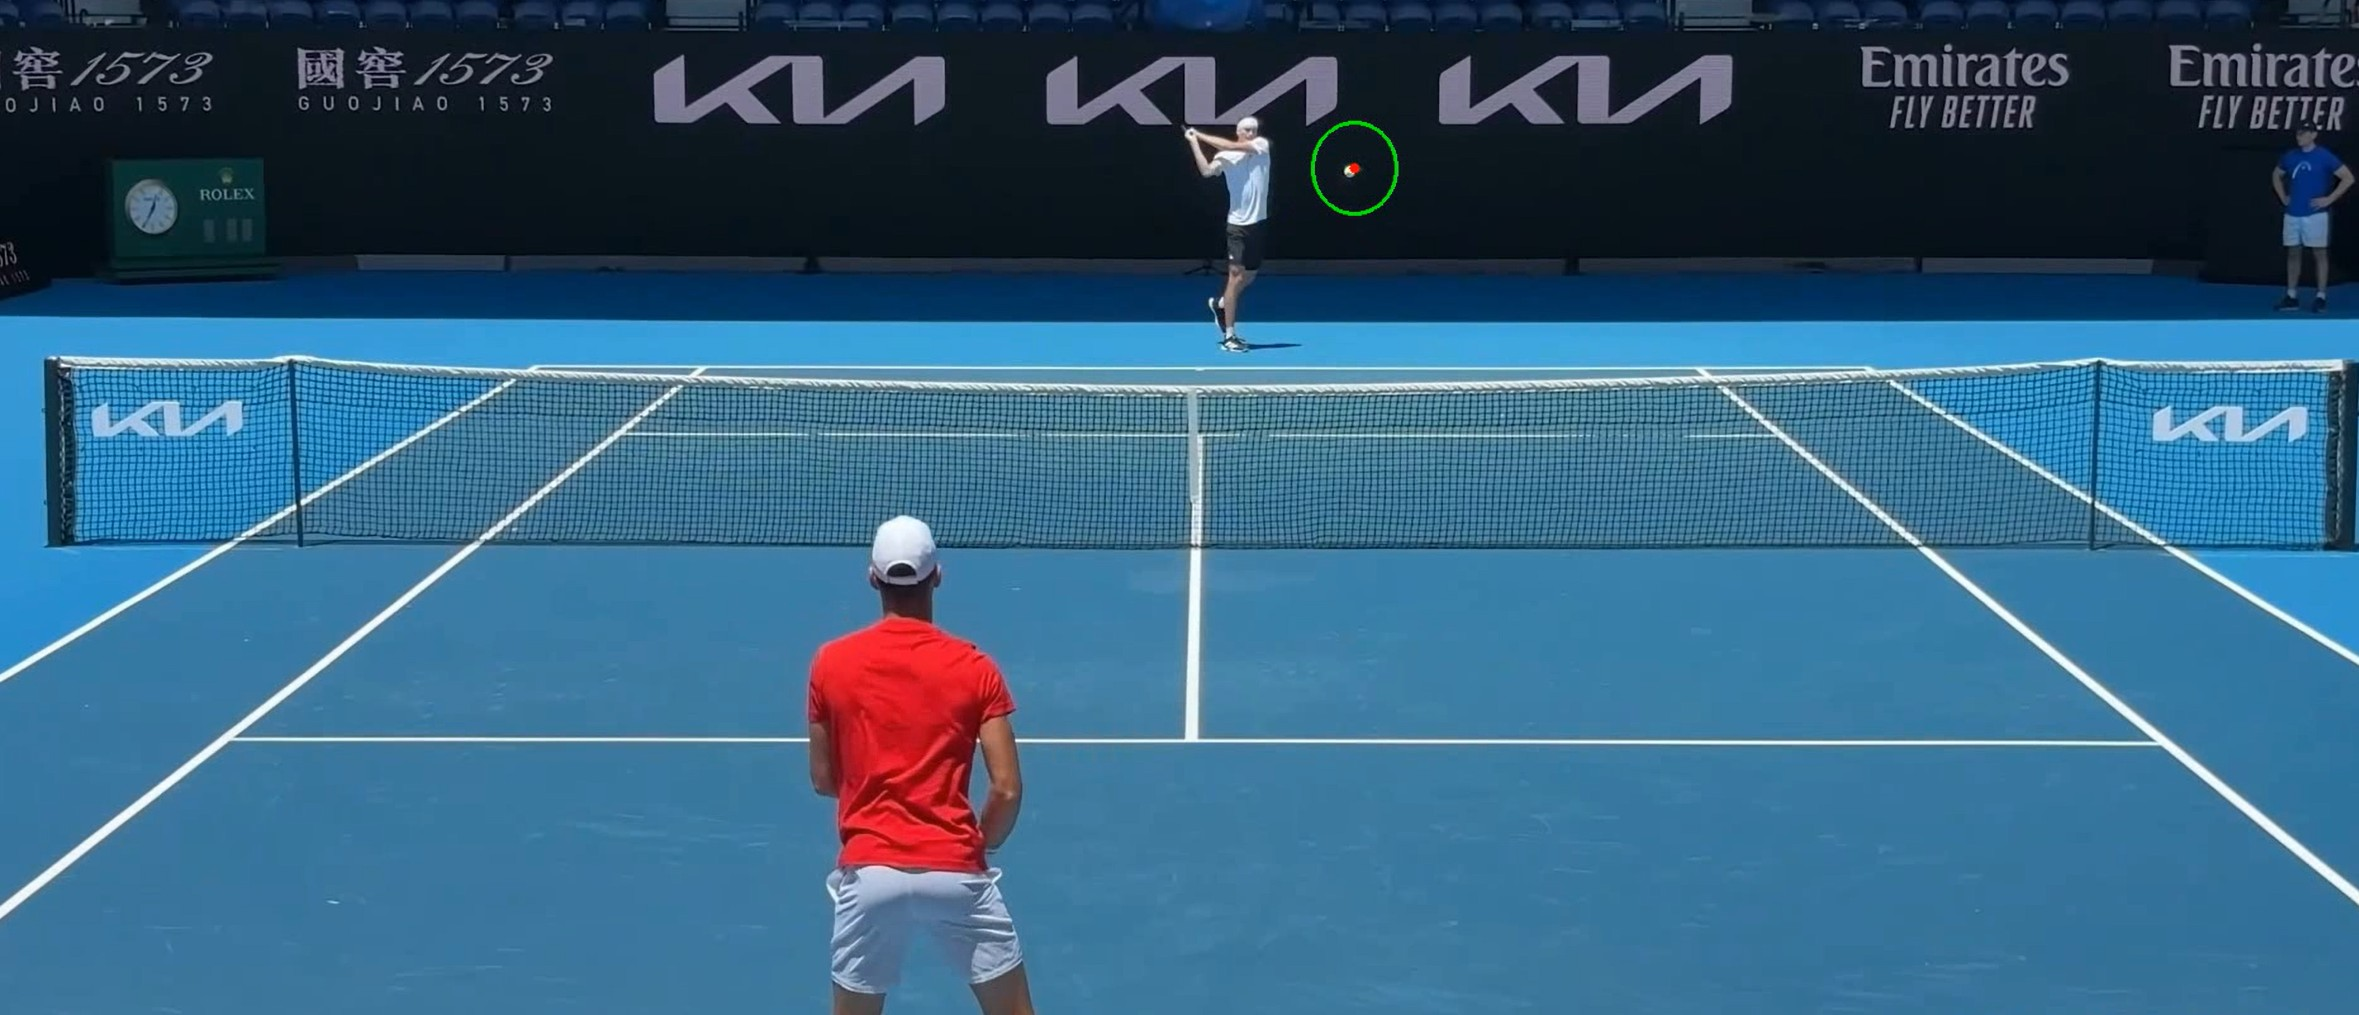
\includegraphics[width=\textwidth]{ZvsDOut.jpg}
	\caption{Example of output from the \acs{pgm} overlayed with the original video footage}
	\label{fig:output}
\end{figure}

\newpage
\section{Evaluation}
This chapter outlines the experimental setup for evaluating the performance of the ball tracking system, focusing predominantly on accuracy and computational efficiency. The chapter begins by describing the datasets and the various inputs required for the system to run, including the video footage and the ground truth data used for evaluation and to ensure reliable benchmarking. This is followed by a discussion of the evaluation metrics used to assess the system's performance, including the accuracy and success rate of the \acs{ipa}, the accuracy of the \acs{pgm} in keeping estimates within a standard deviation of the ground truth, and the overall computational efficiency measured by runtime. The experimental setup is then discussed, detailing the software environment used. The chapter then tunes the parameters of the system to ensure optimal performance. Finally, it concludes with the results and analysis of the system's performance based on the evaluation metrics discussed.

\subsection{Datasets and Inputs}
This section covers the video footage that is used as an input as well as how the ground truth data is generated for evaluation.

\textbf{Video Footage}

The video footage used in this project as described in Section 3.1 is sourced from a YouTube video \parencite{youtube_ZverevDjokovic}, the video is a practice match between Novak Djokovic and Alexander Zverev. The footage is 1080p resolution at 30~\acs{fps} and are cut down to about 15 to 20 seconds long. The frame is 1080x1920 pixels and the camera is static throughout the footage. An example snippet of the footage is shown in Figure~\ref{fig:footage}.

\begin{figure}[H]
	\centering
	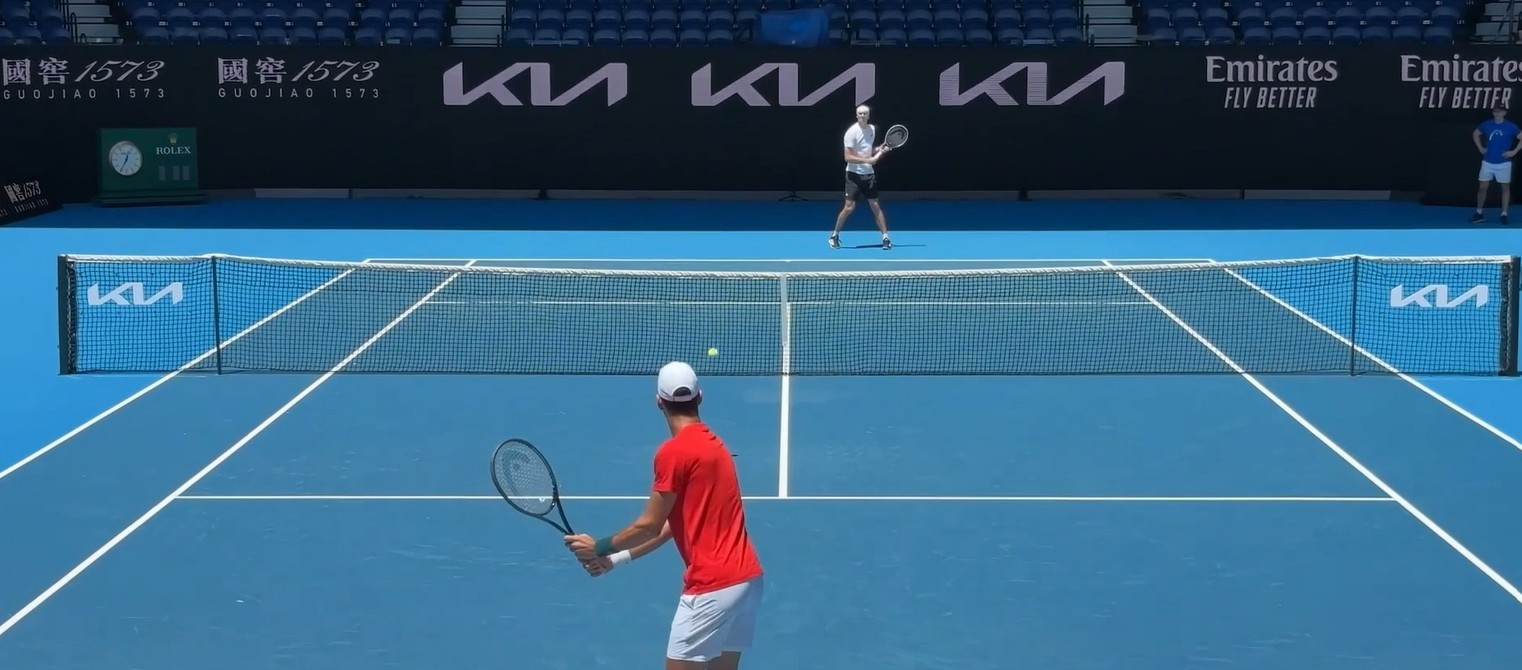
\includegraphics[width=1\textwidth]{ZvDIn.jpg}
	\caption{Example snippet of the video footage used in the project}
	\label{fig:footage}
\end{figure}

The video shows clear lines on the court which is blue and the ball can be see relatively clearly as it is yellow against the background. The footage also shows a variety of ball trajectories, speeds, and occlusions, making it a suitable test case for the tracking system.

The evaluation of the \acs{ipa} and \acs{pgm} will be done using different footage to ensure that the system is robust and can handle various video footage. The ground truth data will be generated for each new footage used in the evaluation.

\textbf{Ground Truth Data}

The ground truth data for the video footage is generated through manual annotation. This is done in a basic Python script, using OpenCV, that allows the user to click on the ball in each frame of the video and then pressing the space bar to move to the next frame. The script also allows the user to skip frames if the ball is not visible, in which case the output for that frame is set to $(-1,-1)$. These recorded positions are then normalized and outputted to a text file called \texttt{groundtruth$\_n$.txt}, the $n$ indicating the specific video footage used. These values will be used to evaluate the performance of the system for both the \acs{ipa} and the \acs{pgm}.

\subsection{Evaluation Metrics}
The performance of all the various systems in the pipeline is discussed in this section. The metrics per system used are discussed in its subsection, that being the \acs{ipa} and the \acs{pgm}.

\subsubsection{\acs{ipa} Evaluation Metrics}
The \acs{ipa} performance is evaluated and selected using two main metrics: Mean Error and Success Rate. This section also details how the Covariance Matrix, and the outlier weights $w_{\pi,a}^{(n)}$ for each \acs{ipa} will be determined for the \acs{pgm}.

\textbf{Mean Error}

The Mean Error is calculated as the average Euclidean distance between the predicted ball position and the ground truth position across all the frames where the ball is visible. This metric providdes a quantitative measure of the accuracy of each algorithm. The formula for Mean Error is given in Equation 34.

\begin{equation}
\text{Mean Error} = \frac{1}{N} \sum_{i=1}^{N} \sqrt{(x_i - x_{gt,i})^2 + (y_i - y_{gt,i})^2}
\end{equation}

where:
\begin{itemize}
	\item $N$ is the number of frames where the ball is visible.
	\item $(x_i, y_i)$ is the predicted position in frame $i$.
	\item $(x_{gt,i}, y_{gt,i})$ is the ground truth position in frame $i$.
\end{itemize}

\textbf{Success Rate}

The success rate of each of the \acs{ipa} is calculated as the percentage of frames where the algorithm successfully detects the ball. Therefore a predicted position of (-1,-1) is considered a failure and any other position is considered a success. The formula for Success Rate is given in Equation 35.

\begin{equation}
\text{Success Rate} = \frac{\text{Number of Successful Detections}}{N} \times 100\%
\end{equation}

\textbf{Covariance Matrix and Weights Determination}

The ground truths data will be compared with the outputs of each algorithm to determine an objective measure for determining the Covariance Matrix which will be used in the \acs{pgm}. This will be done by calculating the standard deviation in the $x$ and $y$ positions and then taking the standard deviation, getting the variances using ($sd^2 = \sigma$) and using it to construct the covariance matrix, where $\sigma_{xx}$ and $\sigma_{yy}$ are the variances of the $x$ and $y$ positions, respectively. The covariance matrix $\Sigma_n$ for algorithm $n$ is defined in Equation 36. This will all be done on a Python script.

\begin{equation}
\Sigma_n = \begin{bmatrix}
\sigma_{x,x} & \sigma_{x,y} \\
\sigma_{y,x} & \sigma_{y,y}
\end{bmatrix}
\end{equation}

The weights will be calculated based on the success rate of each \acs{ipa}. The weight for the inlier component $w_{\pi,inlier}^{(n)}$ will be set to the success rate of algorithm $n$, while the weight for the outlier component $w_{\pi,outlier}^{(n)}$ will be set to $1 - w_{\pi,inlier}^{(n)}$. This ensures that algorithms with higher success rates have a greater influence on the final position estimate, while those with lower success rates are more likely to be treated as outliers.

\subsubsection{\acs{pgm} Evaluation Metrics}
The \acs{pgm} performance is evaluated using two main metrics: Standard Deviation Accuracy and Computational Efficiency. This subsection also highlights the parameter tuning process used to optimize the \acs{pgm} performance.

\textbf{Standard Deviation Accuracy}

The Standard Deviation accuracy metric evaluates how well the \acs{pgm} maintains the estimated ball position within one standard deviation of the ground truth. This metric is calculated by taking the Euclidean distance between the mean of the \acs{pgm} output and the ground truth positions. This distance is then compared with the standard deviation and if it falls within this range it is considered a success, these successes are all summed together and divided by the total number of frames to get the percentage of accuracy. The formula for Standard Deviation Accuracy is given in Equation 37.

\begin{equation}
\text{Std Dev Accuracy} = \frac{\text{Number of Frames within 1 Std Dev}}{N} \times 100\%
\end{equation}

\textbf{Computational Efficiency}

The computational efficiency of the entire system is measured by the runtime of the system after everything has been processed. This is done by measuring the time taken from start to end and is done entirely in code. The runtime is measured in seconds and the aim is to get the runtime to be as close to the actual length of the video footage as possible.

\subsection{Experimental Setup}
The experimental setup for Evaluating the system is done using Ubuntu 24.04.2 LTS on a computer with a 12th Gen Intel Core i5-12450H and 32Gb of RAM. 

\subsubsection{\acs{ipa} Experimental Setup}
In order to evaluate the performance of each \acs{ipa}, each algorithm is run independently with the 1st video footage. This is done to judge the Mean Error and Success Rate of each of the algorithms.

\newpage
\section{Conclusion}
This chapter summarizes the key findings from the project, reflecting on the effectiveness of the proposed ball tracking system. It discusses the strengths and limitations of the approach, as well as potential areas for future work and improvements. The conclusion aims to encapsulate the overall contributions of the project to the field of sports analytics and computer vision. (this still needs to be completed, will emphasize more on what was said in the opening paragraph).

\newpage
\printbibliography
\end{document}